\chapter{Numerical Study of Motion Compensation}


In the previous chapter of this thesis a motion compensation algorithm is proposed as a general algorithm, and then is specifically focused for IGRT. The method however is scarcely compared with standard IGRT 4D CBCT image reconstruction methods, and some questions about the reliability of the motion models arise. Obtaining accurate motion description of the patients is still one of the biggest challenges in 4D imaging, regardless of the method used. How accurate do this models need to be? Additionally, if the motion is previously known to high accuracy, is 4D imaging necessary at all? 

This chapter looks more specifically at these challenges and compares the motion compensated reconstruction to the now most commonly used methods in clinical IGRT. The aim of the work here is to supplement Chapter \ref{ch:motion} with further observations about the behaviour of the algorithm under less ideal numerical data.

The objectives of this chapter are twofold: Firstly, the improved image quality obtainable by iterative algorithms is highlighted, showing how 4D CBCT binning methods can be improved by using better reconstruction algorithms, even with low data. Secondly, the flexibility and error behaviour of the algorithm is studied. The algorithm will reconstruct the image without any motion artefacts if the motion is perfectly know, however respiratory motion is variable between patients and within the patients themselves. The error behaviour with uncertainties in the DVF crucial for the future possibility of the method in clinical cases, as while the motion correction method removes almost in its entirety any motion artefacts with very accurately known DVFs, obtaining very accurate motion models of patients is not possible. Thus, the performance of the method with low resolution and approximately accurate DVFs is studied in this work. Additionally, some proposed methods for 4D CBCT rely in computing DVFs and then deforming a high resolution image with them. This work also studies why using reconstruction for motion correction produces better results than deforming a static image.



\section{Materials and methods}

An small introduction of the POPI dataset, reconstruction methods, methods for deformation vector field computation an reconstructed image quality evaluation parameters are described in this section. 






\subsubsection{4D POPI model}

The dataset that is going to be used is the same as in the previous chapter, a 4D-CT (10 bins) treatment planning scan of a lung cancer patient, known as the POPI model. In Figure \ref{fig:POPIfull} a snapshot of the whole breathing pattern can be seen in the cranial-caudal direction, with a zoomed section of the tumour, on where the motion is better appreciated. Figure \ref{fig:POPI3} shows the only frames 0, 3 and 6, for an amplified image.

\begin{figure}
\begin{center}

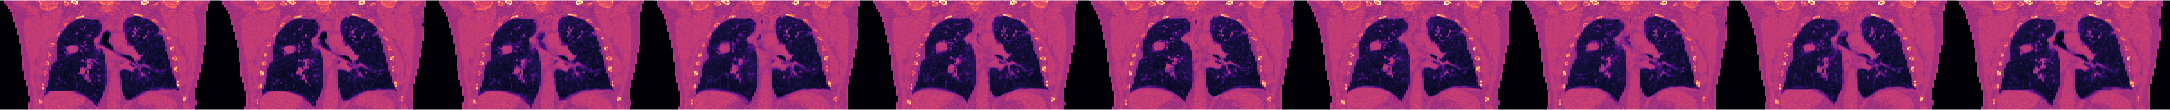
\includegraphics[width=\textwidth]{accuracyMC/imagerall.png} 
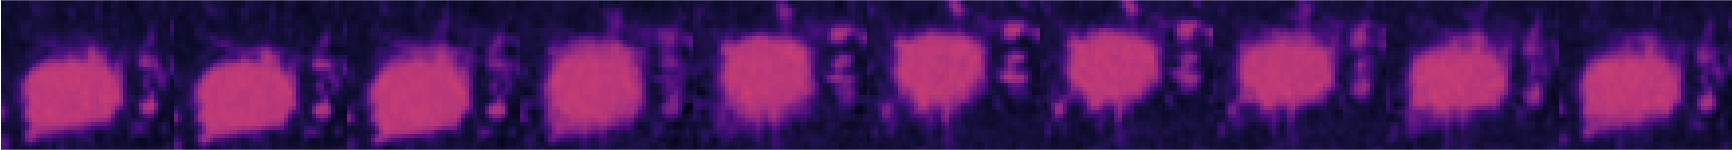
\includegraphics[width=\textwidth]{accuracyMC/tumourall.png} 


\end{center}

\caption[The whole 4D dataset in CC direction]{\label{fig:POPIfull} The POPI dataset for all frames in the cranial-caudal direction, and a zoomed area of the tumour.  The colour scale is linear attenuation coefficient in the range [0-2000].} 
\end{figure}
\begin{figure}
\begin{center}

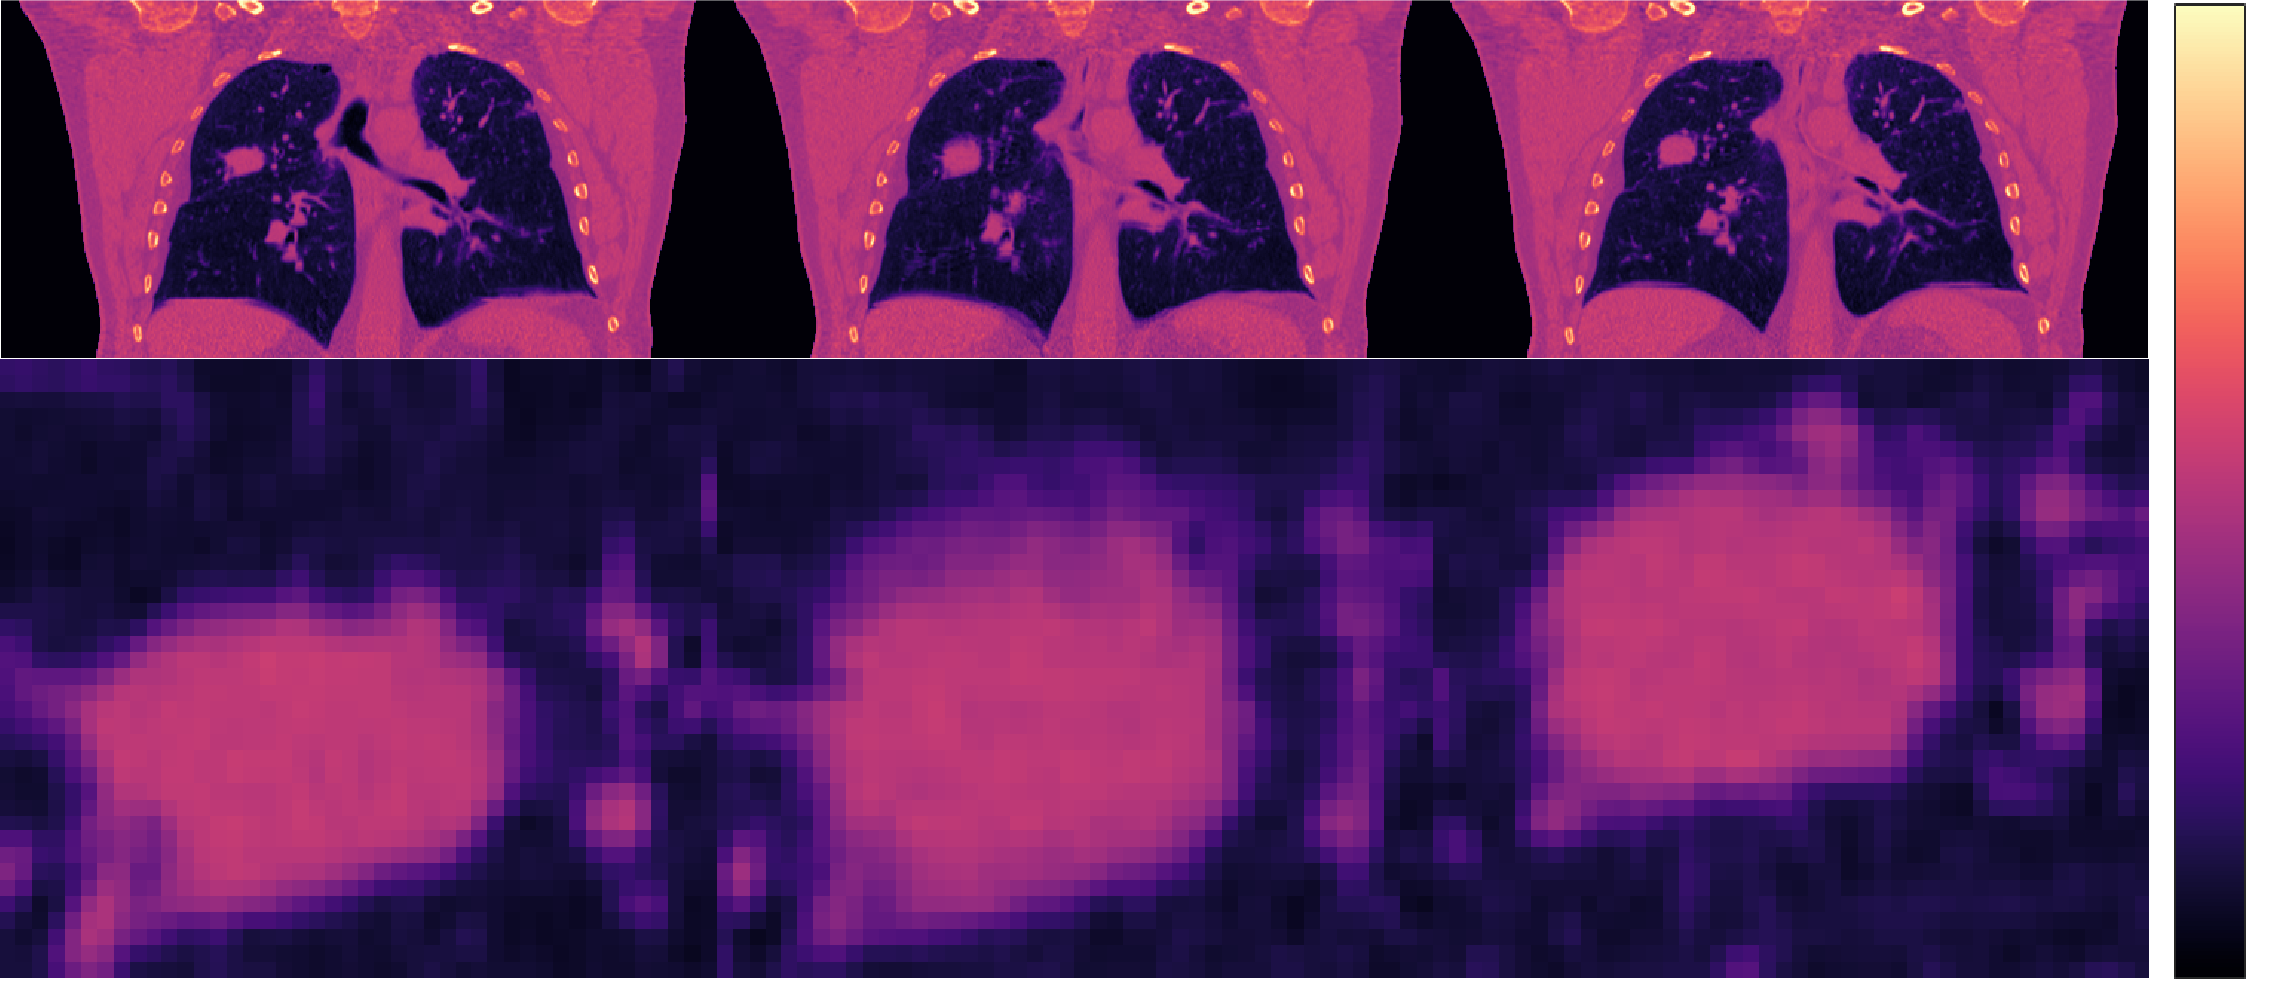
\includegraphics[width=0.9\textwidth]{accuracyMC/imager3.png} 
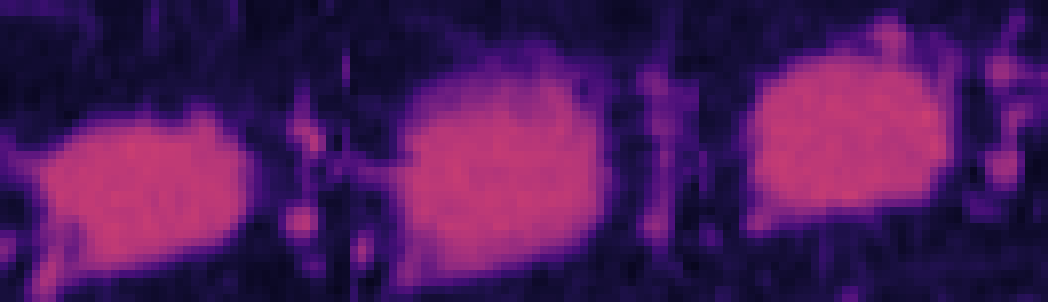
\includegraphics[width=0.9\textwidth]{accuracyMC/tumour3.png} 


\end{center}

\caption[Three frames of the 4D dataset in CC direction]{\label{fig:POPI3} The POPI dataset for three frames (0,3 and 6) in the cranial-caudal direction, and a zoomed area of the tumour.  The colour scale is linear attenuation coefficient in the range [0-2000].} 
\end{figure}

\subsubsection{Image reconstruction}

This chapter reconstruct 4D images in all frames, and compare them to the ground truth. The iterative algorithms used in this section are SART and ASD-POCS. The rationale is that to demonstrate the flexibility of the method, more than one algorithm is presented, and SART is chosen because its a well understood and common algorithm, while ASD-POCS is chosen because its a more advanced algorithm with more complex constrains, however it is also quite well known one. One would expect that more advanced and newer algorithms to work even better than these two, but using those may obscure the results of the analysis that this chapter attempt to study, the quality of the reconstruction with the common errors in 4D CBCT.

\subsubsection{Deformation vector field computation}

As images in all frames are reconstructed in this chapter, deformation fields from and to any arbitrary time snapshot are required by the algorithm. For 10 frames, this makes 90 deformation vector fields + 10 identity fields (all zeroes). The DVfs used in the previous chapter that are provided with the POPI model only register to a single time slice (the second one, labelled 1), thus they are not enough to reconstruct the data in this chapter. In order to obtain the needed DVFs, a third party software has been used, the Elastix\cite{elastix} package. Elastix is an open source software that provides a big variety of multimodal nonrigid image registration tools. 

From the algorithms available in the package, a nD+t B-spline group-wise cyclic registration\cite{metz2011nonrigid} approach has been chosen. This method is an optimization based algorithm, that registers 4D images (in this case) with B-splines. This allows for an analytic representation of the deformation using a simple yet fast method. The algorithms assumes deformation only in the spacial domain, and smoothness, as it is mean to represent intra-patient deformation. An assumption is made that a correctly registered image should have the same pixel intensity value in each corresponding spacial location, thus a cost function of the following form is defined:

\begin{equation}
C(\mu)=\frac{1}{\lVert \mathcal{S} \rVert\lVert \mathcal{T}\rVert}\sum_{x\in \mathcal{S}} \sum_{t\in\mathcal{T}}\left(I(T_\mu(x,t)) - \bar{I_\mu}(x)\right)^2,
\end{equation}
where $I$ is a n-dimensional image, $\bar{I_\mu}(x)$ is the average intensity value over time (after applying the transformation), $T_\mu(x,t)$ is the B-splice coordinate transformation, $\mu$ the B-spline parameters, and $\mathcal{S}$ and $\mathcal{T}$ the set of spacial and temporal coordinates respectively. As multiple solutions exist for this equation, an additional constrain is added. As the registration is cyclical, a constrain in the coordinate transformation is added, that the average transformation must be the identity, as in
\begin{equation}
\frac{1}{\lVert \mathcal{T}\rVert}\sum_{t\in\mathcal{T}}T_\mu(x,t)=x.
\end{equation}

The minimization equation therefore is
\begin{equation}
\hat{\mu}=\argmin_\mu C(\mu) \text{  subject to  } (7.2).
\end{equation}

This equation is minimized using adaptive stochastic gradient descend, a faster converging version of gradient descend\cite{klein2009adaptive}. For more details about the specific implementation, refer to the article\cite{metz2011nonrigid}.

This algorithm needs an initial grid of spatial points to register and link via B-splines. The grid size used in this work is an uniformly distributed grid with samples every 13x13x1 voxels.
\subsubsection{Quantitative reconstruction quality parameters}

To evaluate the quality of the reconstruction, the tumour is going to be the focus, as  in the previous chapter. The metrics RMSE and UQI and Segmentation mismatch will also be used, however an additional metric to compute the binary shape location of the tumour will also be used.  Using the same tumour area, the tumour will be extracted using morphological operators on images, via binarization with Otsu's method, image dilation and erosion and labelling using connected components. The biggest segmented blob will be then used to compute the geometric center, and the euclidean distance between this and the ground truth will be used as metric of quality. This is due to CBCT not reconstructing HU units of images with the best accuracy, thus the quality of the result on image attenuation coefficient values is less important than the quality of the shape of the tumour. The attenuation coefficients are actually important for RT planning, however CBCT is mainly used to know the tumour shape and location on the treatment.




\section{Results}

In order to evaluate the flexibility of the motion compensated iterative algorithms various numerical test are performed and the qualitative parameters computed in the results. The first test shows the quality of using iterative algorithms versus FDK in 4D CBCT applications, without motion compensation. Then the motion compensated method will be compared to 4DCBCT, using only a tenth of projections. The lasts tests will focus on DVFs and quality of DVFs. Three different studies are presented. The first shows the effect of a highly under-sampled DVF, the second reconstruct images with 10\% of the projections being labelled in the wrong bin (thus using the wrong DVFs) and the last one tests the reconstruction quality in case where DVFs are only available for the tumour area. Comparison to the 3D CBCT image with motion artefacts is not performed in this chapter, needless to say it performs worse than the motion compensation algorithms in all cases except on frame number 4, on where the tumour average lies approximately, thus locating its centroid with the same accuracy as motion compensated methods.

\subsection{Iterative algorithms vs FDK in 4D CBCT}
The standard procedure for a 4D CBCT image used currently in the clinic is to obtain projections of the patient breathing of the order of 1000-1600\cite{thengumpallil2016difference} projections per session while monitoring the breathing phase with some external surrogate. Then the projections are binned for each breathing phase (generally 6-10 different phases) and the images are reconstructed for each bin, with the FDK algorithm. For an dataset of 100 noiseless projections per bin, where all projections have been perfectly binned, and there is no intra-bin motion, figure \ref{fig:4dCBCT3static} shows the reference images and reconstruction with FDK, SART and ASD-POCS (rows) for bins 0, 3 and 6 (columns), with 50 iterations in the iterative algorithms. The improved quality of the iterative algorithms compared to FDK is clearly visible. This just reafirms the results presented in other studies\cite{schmidt2014clinical}\cite{shieh2014image}, where iterative algorithms have been shown to be superior than FDK in 4D CBCT. Figure \ref{fig:4dCBCTquality} shows the quality parameters computed for the tumour area for each frame and algorithm. Iterative algorithms perform better, ASD-POCS obtaining the best result in almost all parameters.
 
\begin{figure}
\begin{center}

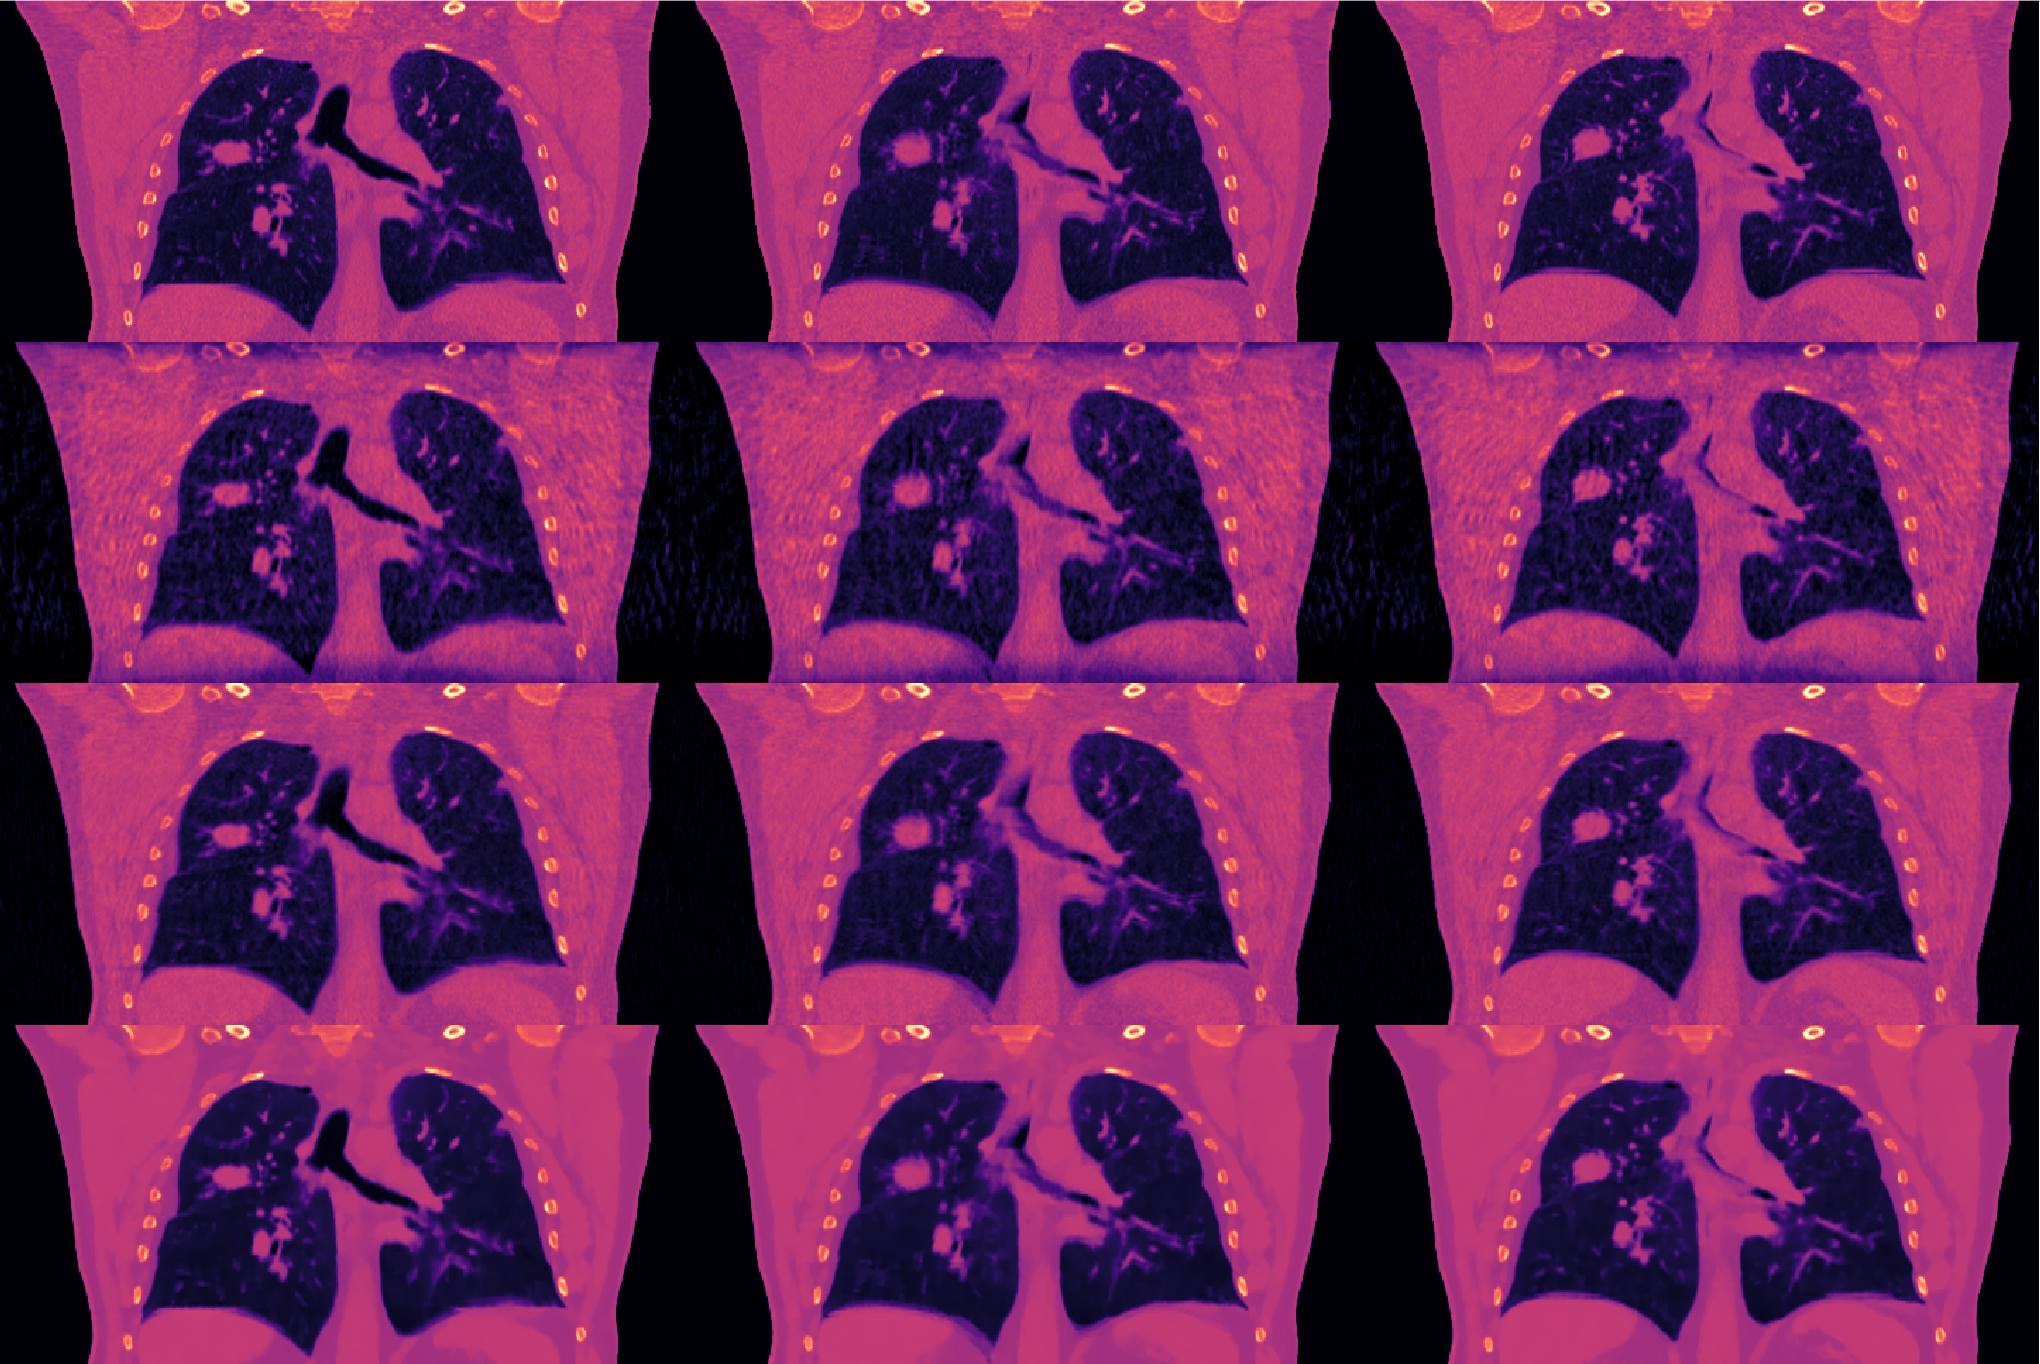
\includegraphics[width=\textwidth]{accuracyMC/4DCBCT3stage.png} 


\end{center}

\caption[Three frames of the 4D CBCT recosntruction with different algorithm]{\label{fig:4dCBCT3static} The POPI dataset for three frames (0,3 and 6) and reconstruction of each frame using 100 projections by FDK, SART and ASD-POCS, from top to bottom.  The colour scale is linear attenuation coefficient in the range [0-2000].} 
\end{figure}

\begin{figure}
\begin{center}

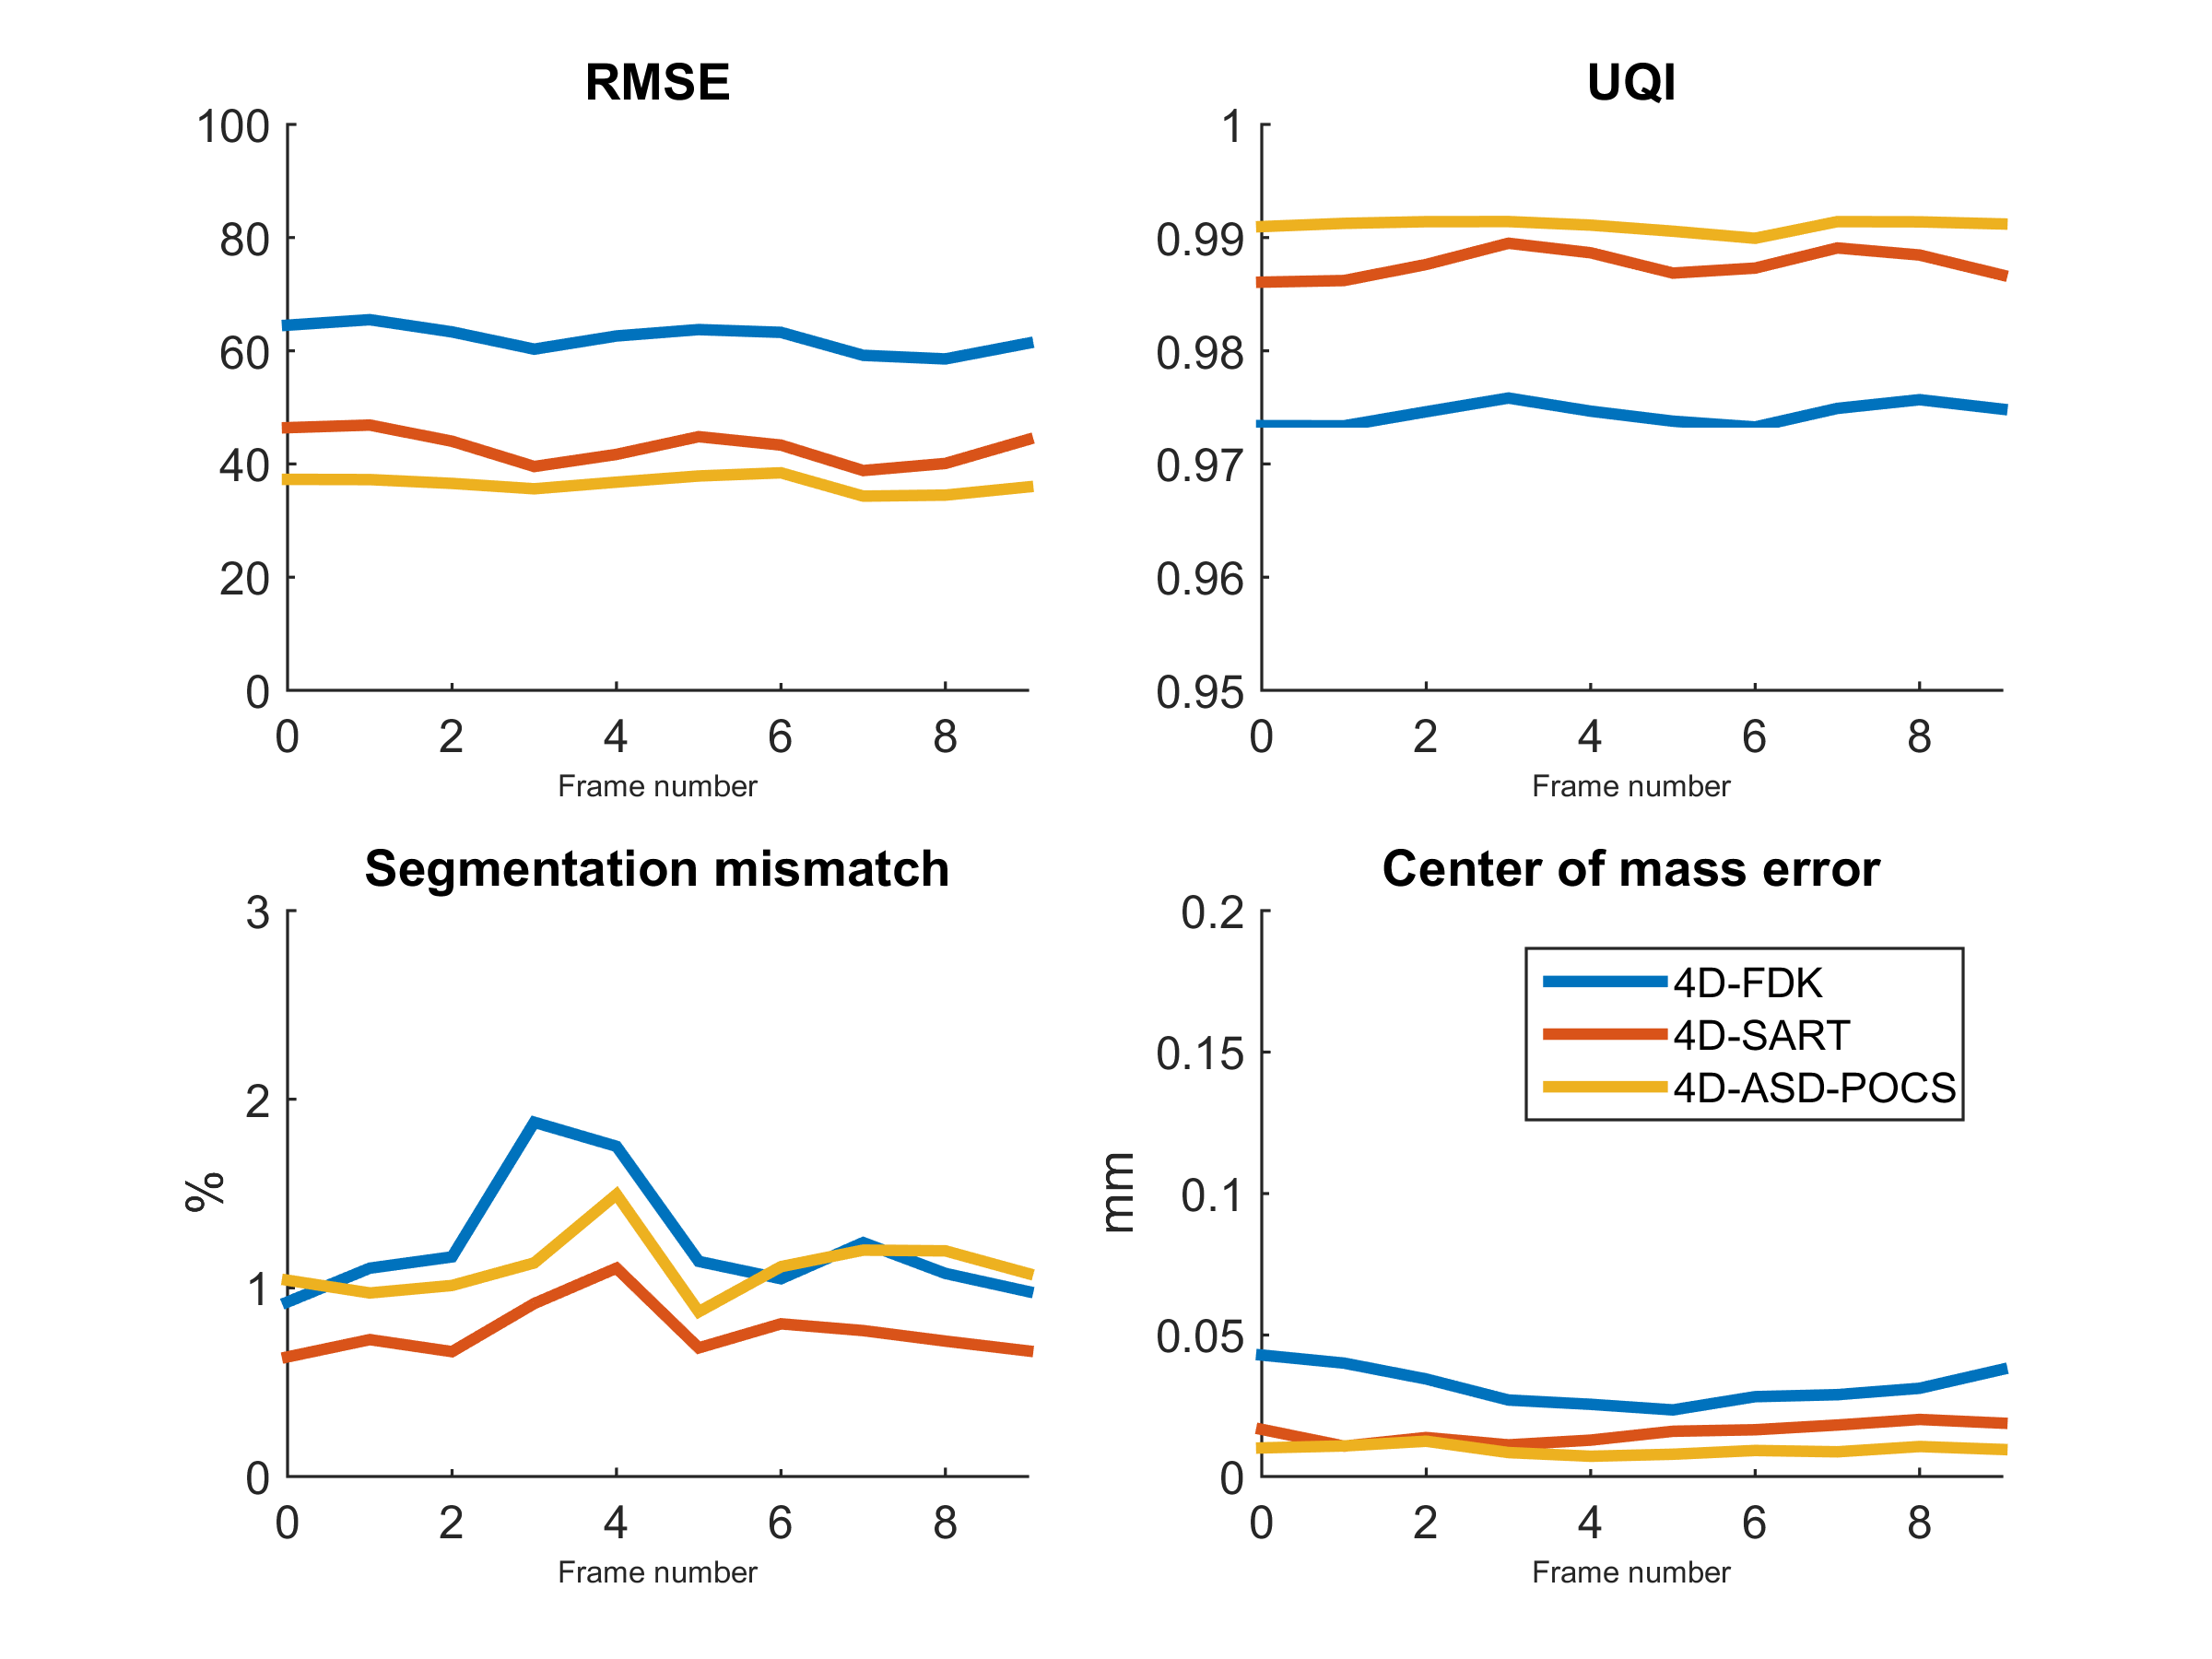
\includegraphics[width=0.9\textwidth]{accuracyMC/4DCBCTparams.png} 


\end{center}

\caption[Reconstruction quality comparison of 4D CBCT algorithms]{\label{fig:4dCBCTquality} Reconstruction quality comparison of 4D CBCT algorithms for each frame. Horizontal axis shows frame number and vertical axis the value of the quality parameter. Iterative algorithms show better performance compared to FDK in all cases.} 
\end{figure}

\subsection{Motion Compensated vs 4D CBCT}

The motion compensated reconstruction is compared to 4D CBCT reconstruction in this section. It is important to remember that the motion compensated reconstruction uses only 100 projections in total, the same projections to reconstruct each of the different frames. In the 4D CBCT algorithms the total number of projections is 1000, binned in 10 frames. Figure \ref{fig:MCCBCT3static} shows the real data, 4D CBCT using FDK and reconstruction using motion compensated algorithms, SART and ASD-POCS respectively. SART has a similar noise level than FDK, while ASD-POCS removes most of that noise. Figure \ref{fig:MCCBCTquality} shows the quality parameters for 4D CBCT FDK, motion compensated SART and ASD-POCS, and the frame number 4 deformed by the DVFs. This last one is presented to present the quality of the DVFs used. While in the real case the original image would be unknown, especially with this quality, its comparison here is of use. The motion compensated algorithms rely in this data, thus in case where the algorithm itself would have no errors and the DVFs would be completely coherent (perfect match on motion from and to the frames) the warped original image would be the best case scenario for the algorithms. These are not the best quality DVFs (e.g. the ones provided with the POPI model for frame number 1 are better), however they are a good example of smooth DVFs that one can obtain in 4DCBCT.

In the results one can see that while the quality of the reconstruction is lower than in 4D-CBCT, it is still good in general terms. The center of the tumour is located within 1mm of error on most cases, less than the error in proton therapy dose delivery. 


\begin{figure}
\begin{center}

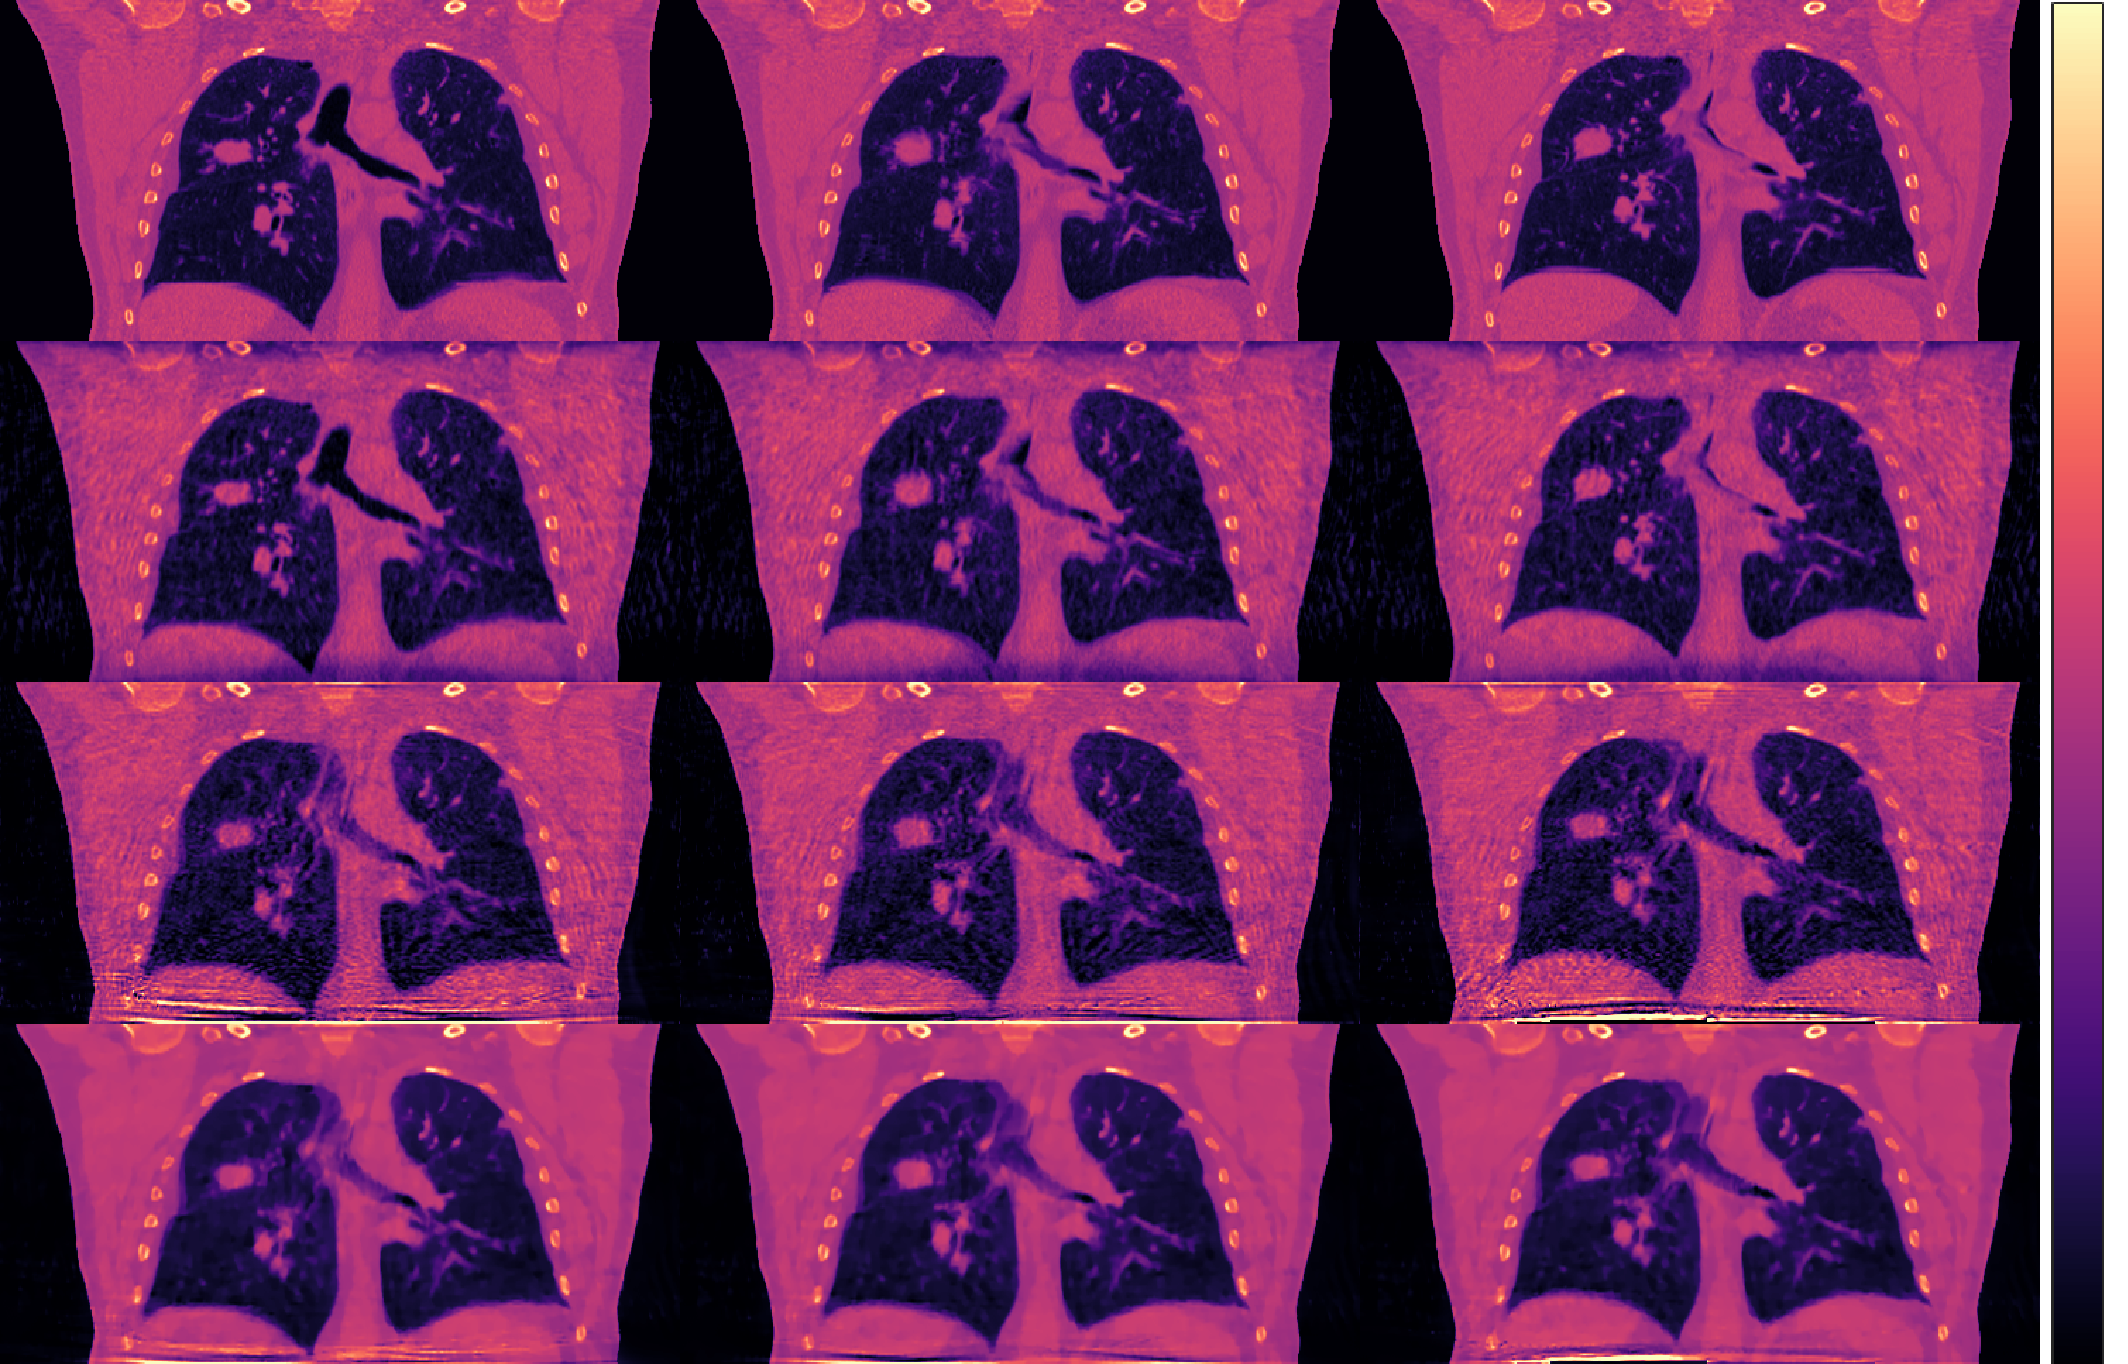
\includegraphics[width=\textwidth]{accuracyMC/MCCBCT3stage.png} 


\end{center}

\caption[Three frames of the motion compensated CBCT recosntruction with different algorithm]{\label{fig:MCCBCT3static} The POPI dataset for three frames (0,3 and 6) and reconstruction of each frame 4D CBCT FDK, motion compensated SART and motion compensated ASD-POCS, from top to bottom.  The colour scale is linear attenuation coefficient in the range [0-2000].} 
\end{figure}

\begin{figure}
\begin{center}

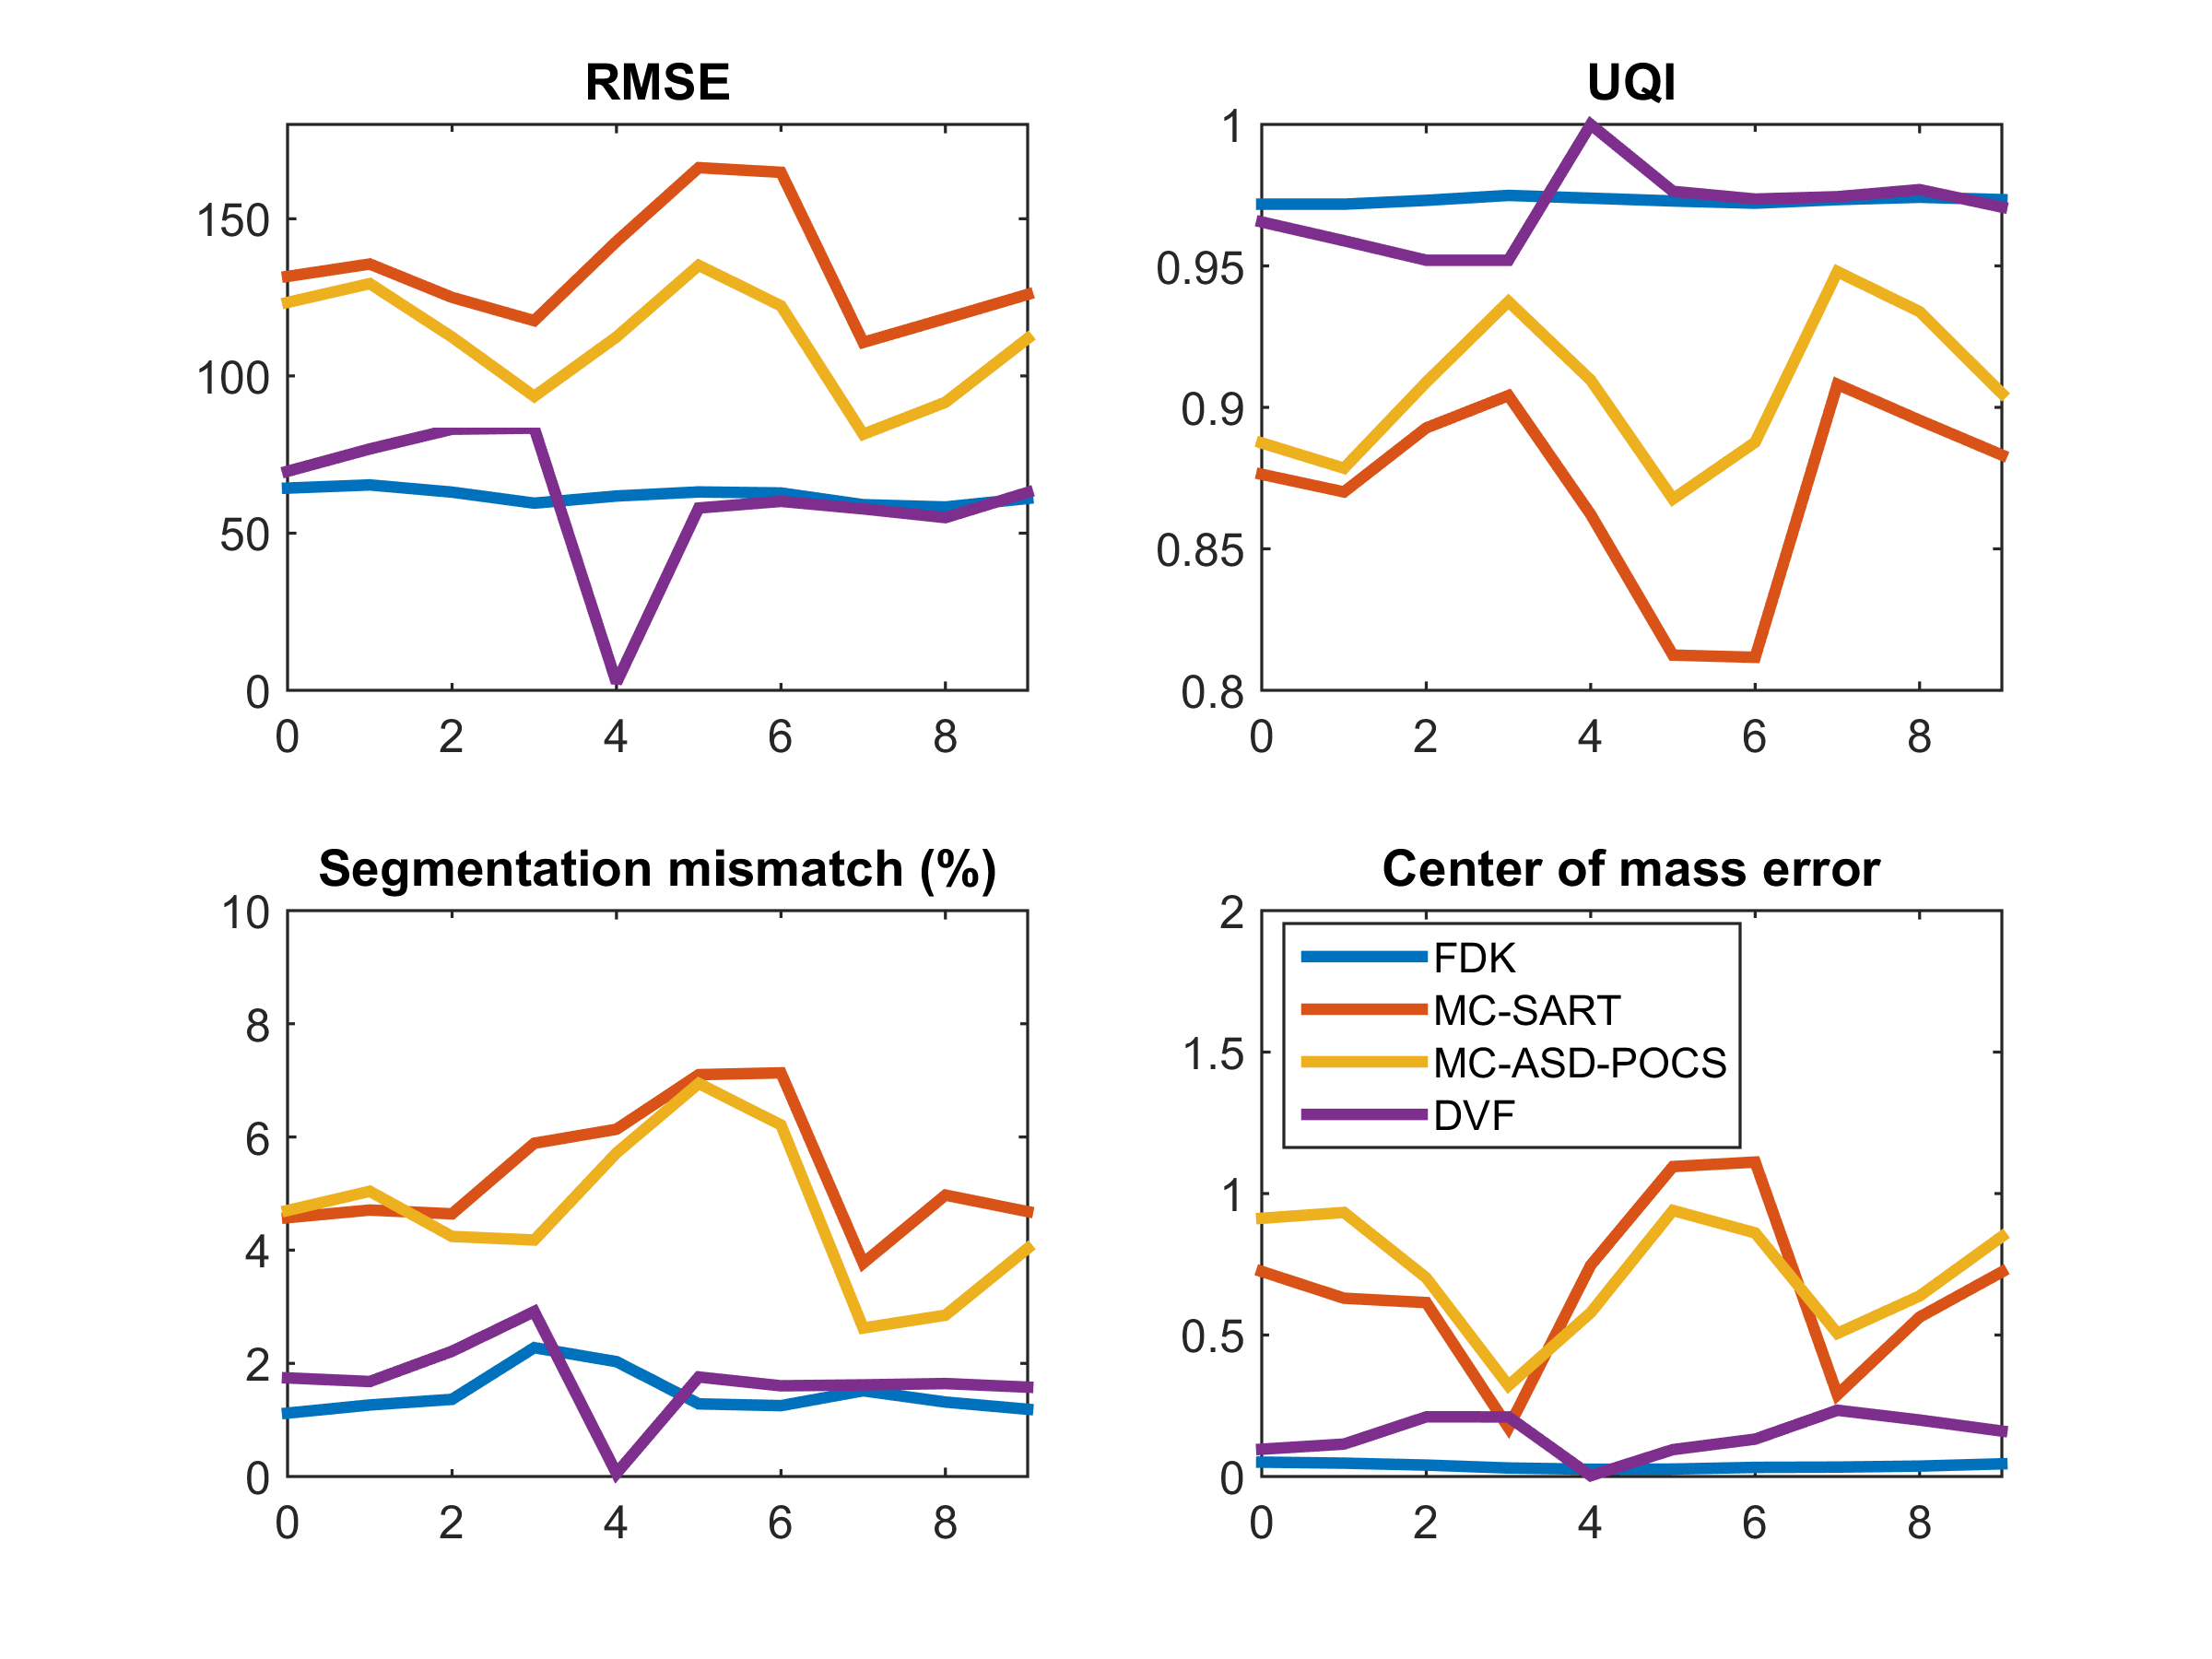
\includegraphics[width=0.9\textwidth]{accuracyMC/MCCBCTparams.png} 


\end{center}

\caption[Reconstruction quality comparison of motion compensation]{\label{fig:MCCBCTquality} Reconstruction quality comparison of 4D CBCT FDK, motion compensated methods (SART and ASD-POCS) and the 4th frame after deformation. Horizontal axis shows frame number and vertical axis the value of the quality parameter.} 
\end{figure}

\subsection{Substandard Deformation Vector Fields}
The biggest single challenge of the motion compensation method is the fact that obtaining accurate patient specific DVFs is not possible with the current methods. Thus, evaluating numerically how accurately the DVFs need to be known for the algorithm to perform within reasonable limits is an important factor. The previous chapter shows that if the DVFs are perfectly known the motion compensated method can completely eliminate the motions influence in the final image, and the first section of this chapter shows that a smooth cyclic DVF computation algorithm can, while with more error, lead to accurate reconstruction. This section pushes the limits of the DVFs numerically in order to evaluate ho much the reconstruction quality deteriorates with each of the effects. The motion compensated methods with full DVFs are taken as a baseline for comparison.

\subsubsection{Undersampled DVFs}
While obtaining accurate DVFs may be a problem, it is easier to obtain broad smooth DVFs in a coarse grid that show roughly the motion of the area. Obtaining these is both numerically robust and  computationally cheap, making it a viable option in a clinical case. While the DVFs computed for the previous sections of chapter have been defined in a 13x13x1 spaced grid, the intermediate points are calculated with B-spline, thus allowing more complex behaviour than with linear interpolation in the intermediate voxels. In this simulation, the DVFs defined voxel by voxel is down-sampled to a 16x16x16 spaced grid, resulting on a 22x30x9 grid, that is linearly interpolated. 

Visually the results are very similar to the full DVF motion compensation method, so the difference between them is visualized in figure XX for SART and ASD-POCS. The quality parameters are compared to the full DVF motion compensation and 4D CBCT FDK in figure \ref{fig:UMCCBCTquality}. In there, while an obvious lower accuracy than the full DVF method is obtained by the undersanpled one, the deterioration is not very significant. The location of the tumour is still below 1.5 mm of error for all frames, around 1mm on average.

\begin{figure}
\begin{center}

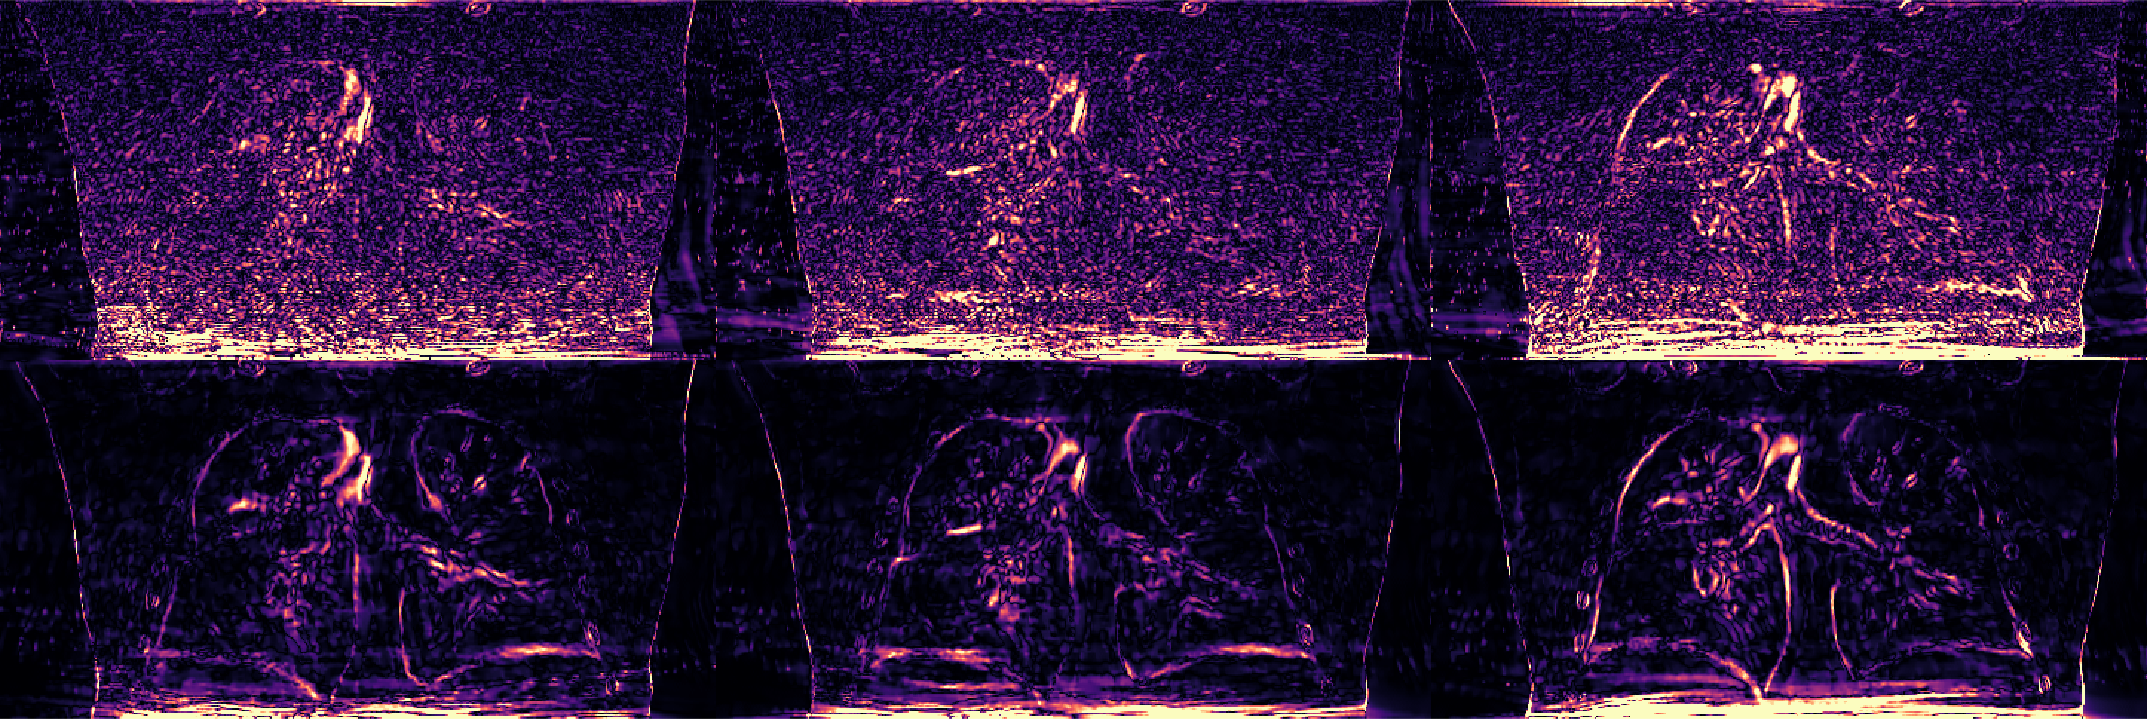
\includegraphics[width=\textwidth]{accuracyMC/diffUMCCBCT3stage.png} 


\end{center}

\caption[Three difference frames of the undersampled motion compensation methods]{\label{fig:UMCCBCT3static} Absolute difference plots in frames (0,3 and 6) for the motion compensation methods with full DVFs and undersampled DVFs, for SART and ASD-POCS, from top to bottom.  The colour scale is linear attenuation coefficient in the range [0-400].} 
\end{figure}


\begin{figure}
\begin{center}

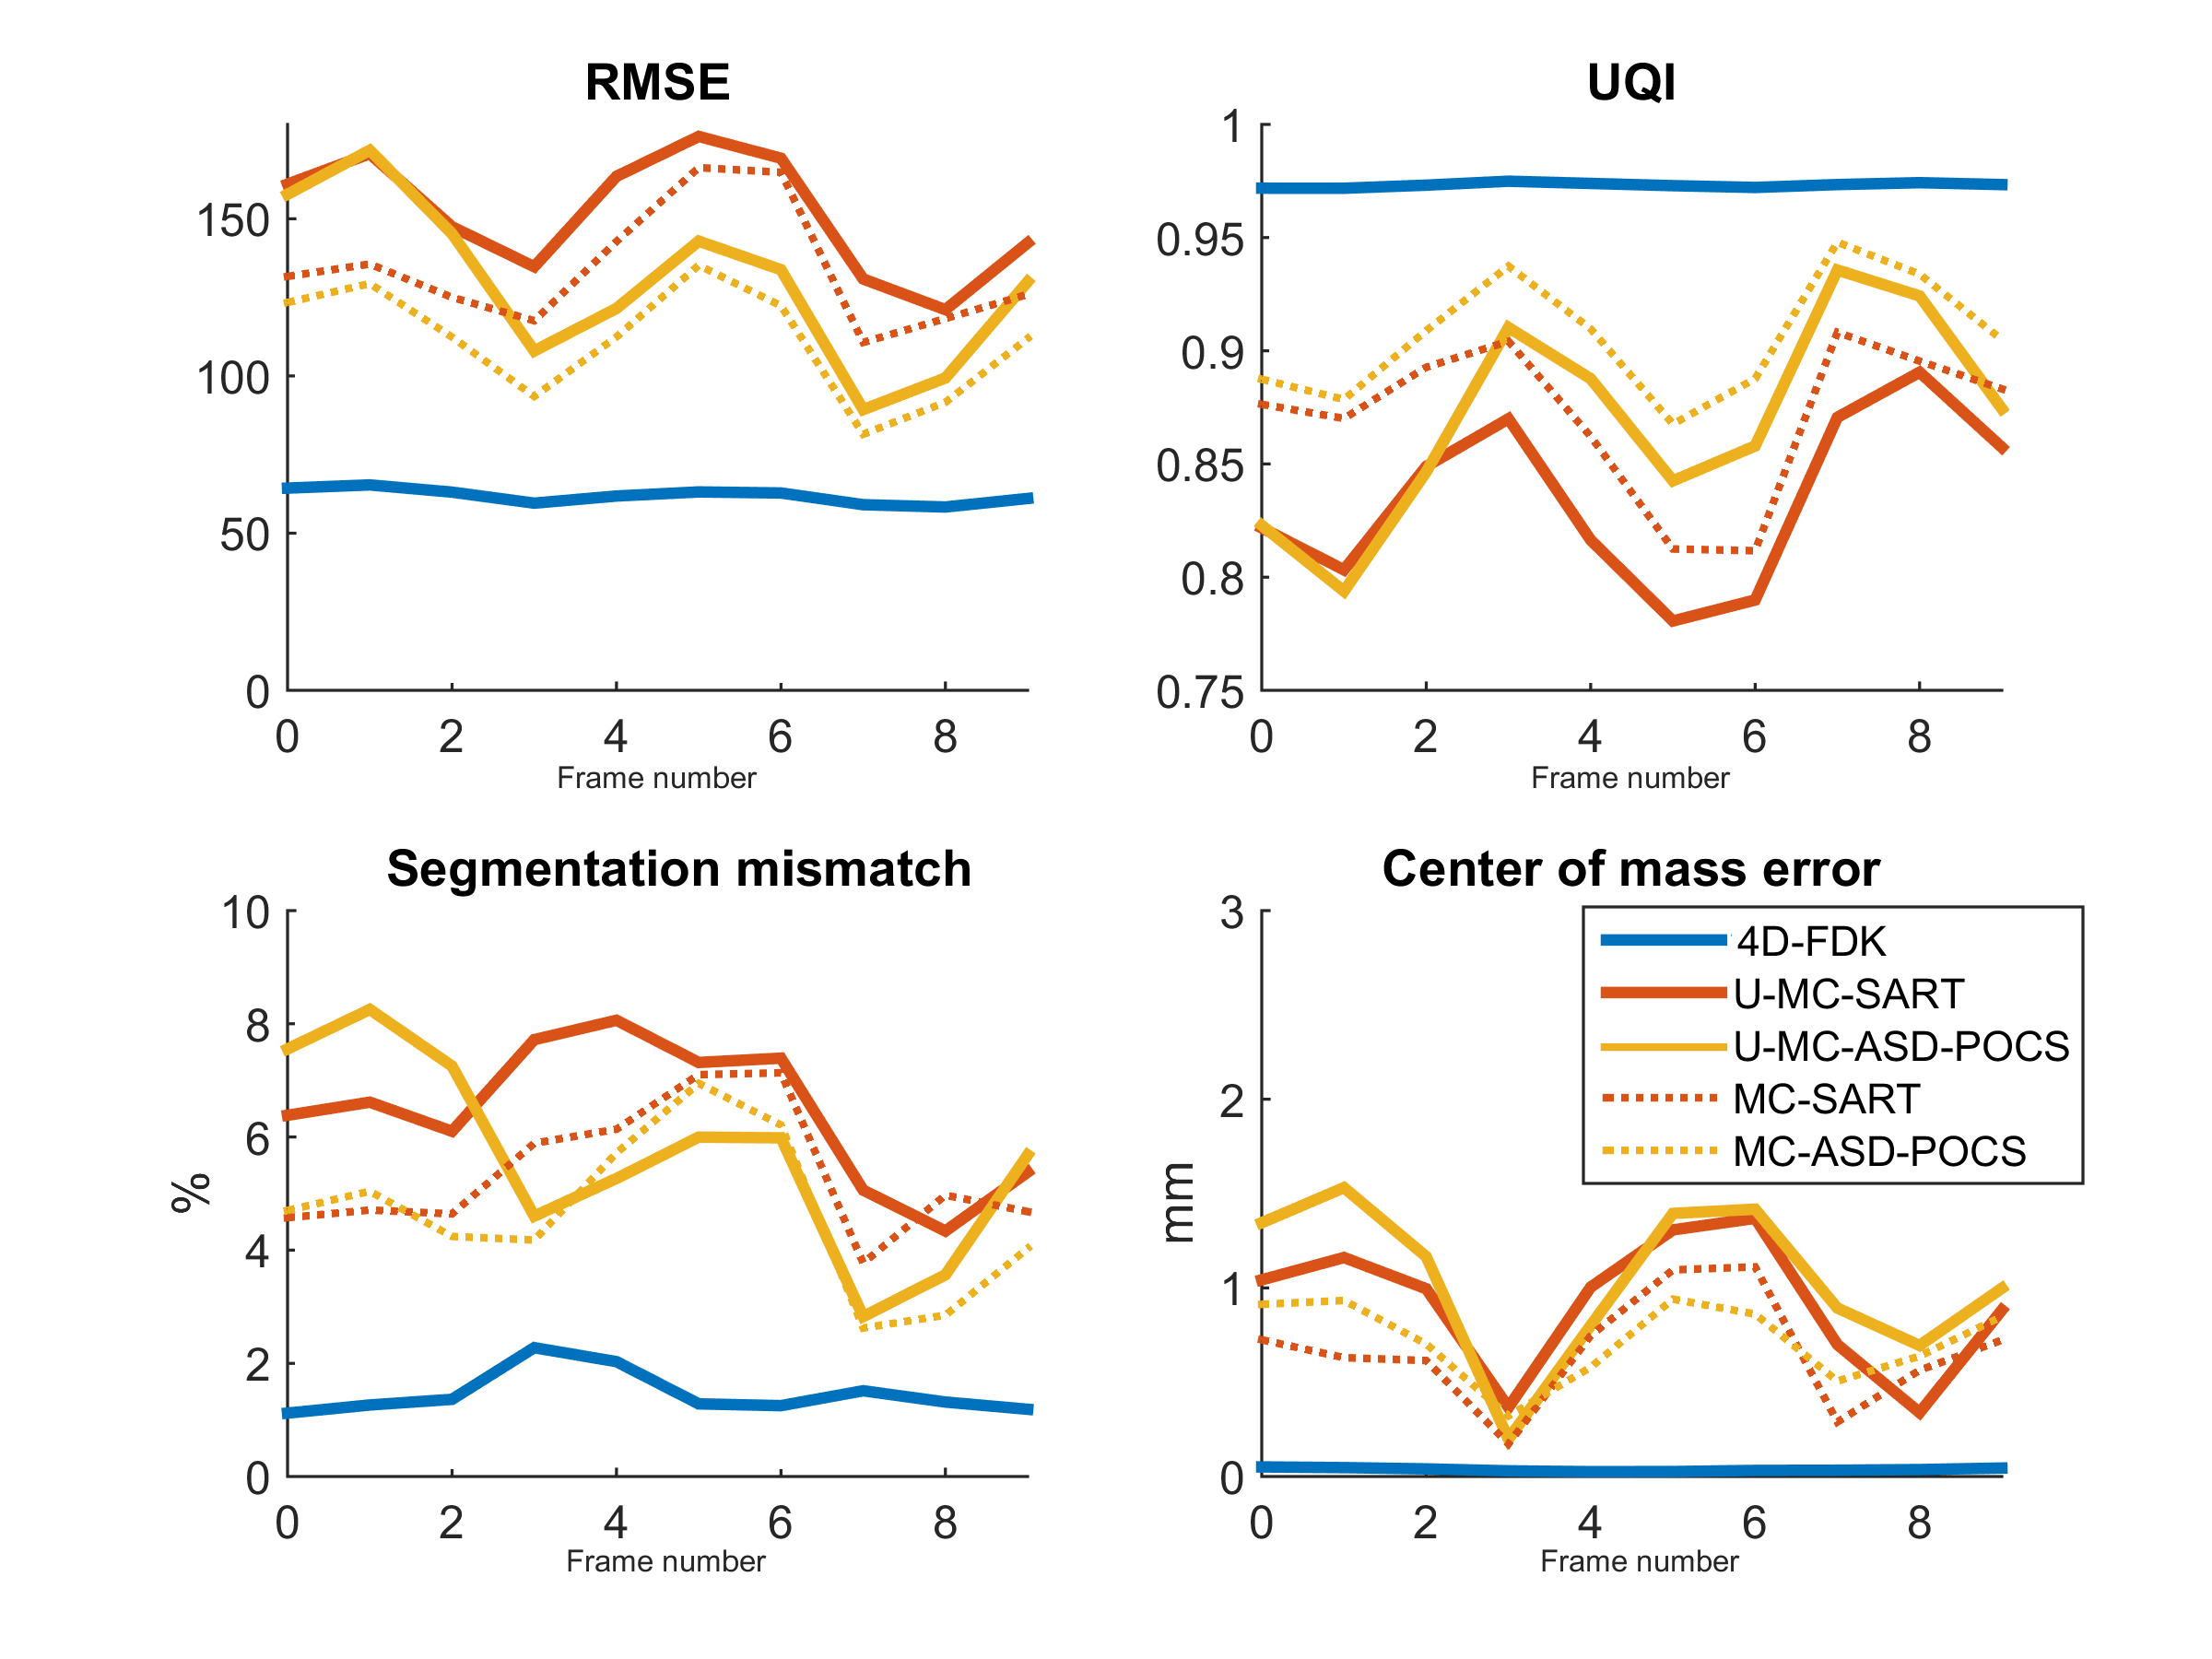
\includegraphics[width=0.9\textwidth]{accuracyMC/UMCCBCTparams.png} 


\end{center}

\caption[Reconstruction quality comparison of motion compensation]{\label{fig:UMCCBCTquality} Reconstruction quality comparison of 4D CBCT FDK, motion compensated methods (MC-SART and MC-ASD-POCS) and motion compensated methods with undersampled DVFs (U-MC-SART and U-MC-ASD-POCS). Horizontal axis shows frame number and vertical axis the value of the quality parameter.} 
\end{figure}
\subsubsection{Binning errors in projections}
Another of the most common errors in 4D CBCT is the mislabelling of projections to the wrong breathing phase. When binning the projection, the breathing surrogates monitoring the phase may fail, either due to inherent unavoidable system errors or because the patient changed its breathing pattern during data acquisition. It is thus often a common error that projections are labelled wrongly, generally by 1 bin (e.g. a projection from phase number 4 is labelled as 3 or 5). In this experiment 10\% of the projections are randomly mislabelled to an adjacent bin, thus using the wrong DVFs in reconstruction. The effects of this mislabelling can be seen in comparison to correct DVFs in figure \ref{fig:binMCCBCT3static} and the quality parameters can be seen in figure \ref{fig:binMCCBCTquality}. The results show that for SART, the error in most parameters increase a bit, however for ASD-POCS, the effect is negligible. This is an expected behaviour, as mislabelling of the projections would lead to a wider transition in tumour edges, however the total variation algorithm does sharpen smooth edges, thus removing this effect.


\begin{figure}
\begin{center}

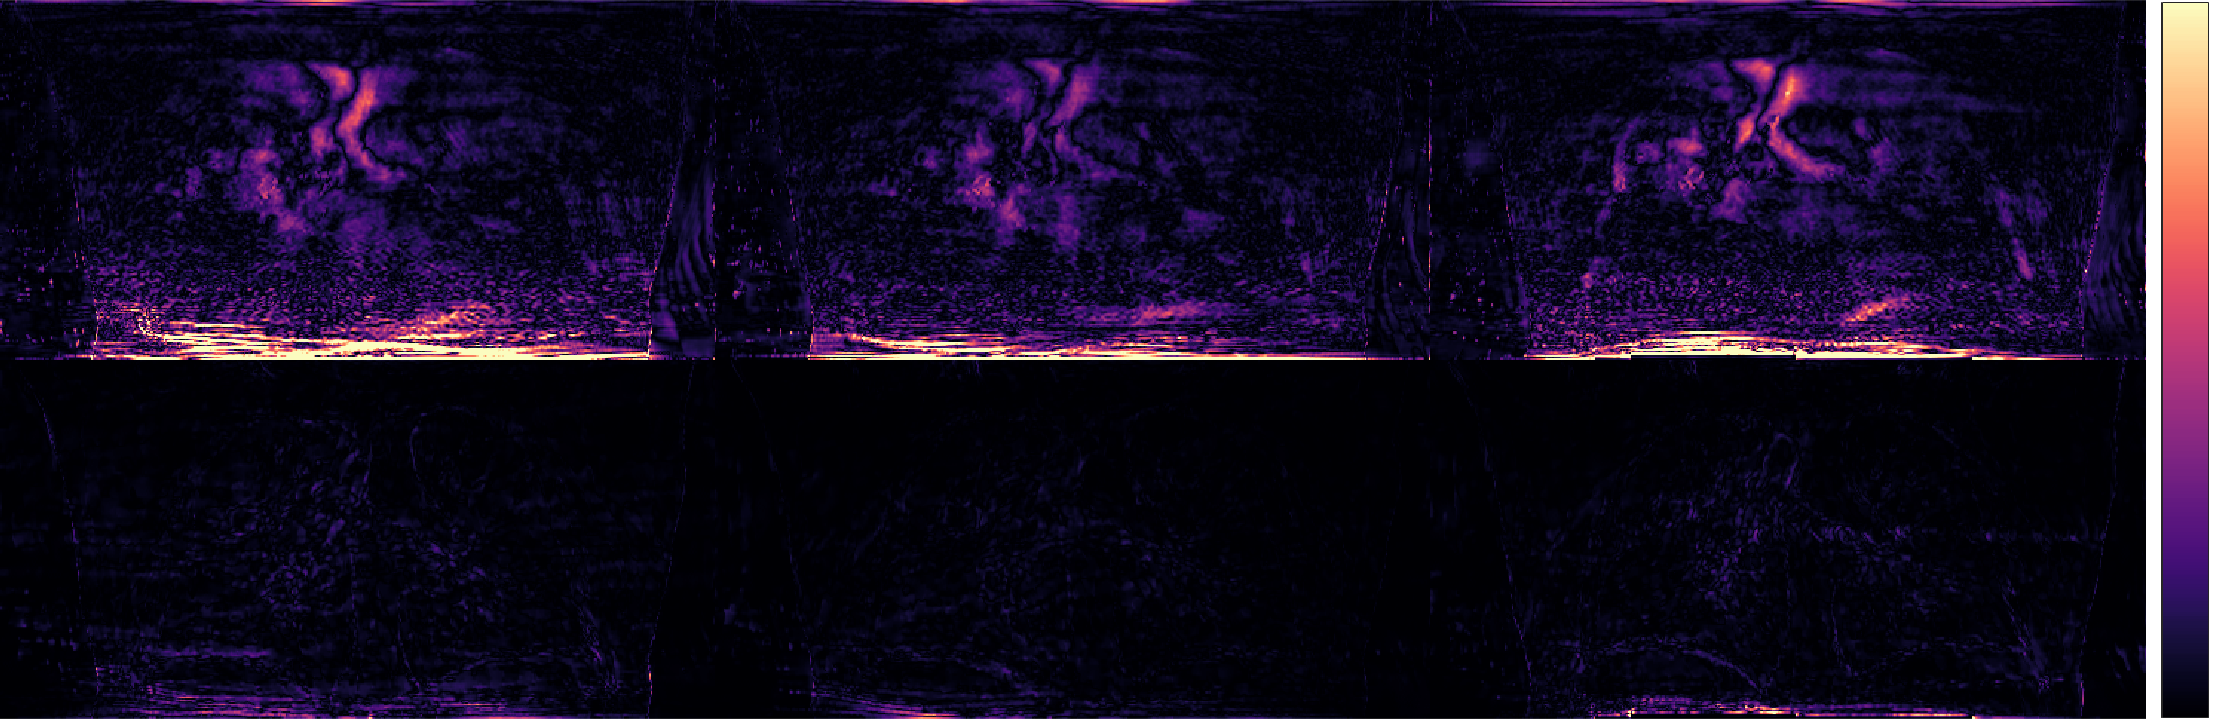
\includegraphics[width=\textwidth]{accuracyMC/diffbinninMCCBCT3stage.png} 


\end{center}

\caption[Three difference frames of the  motion compensation methods with projection binning errors]{\label{fig:binMCCBCT3static} Absolute difference plots in frames (0,3 and 6) for the motion compensation methods with and without binning errors, for SART and ASD-POCS, from top to bottom.  The colour scale is linear attenuation coefficient in the range [0-400].} 
\end{figure}


\begin{figure}
\begin{center}

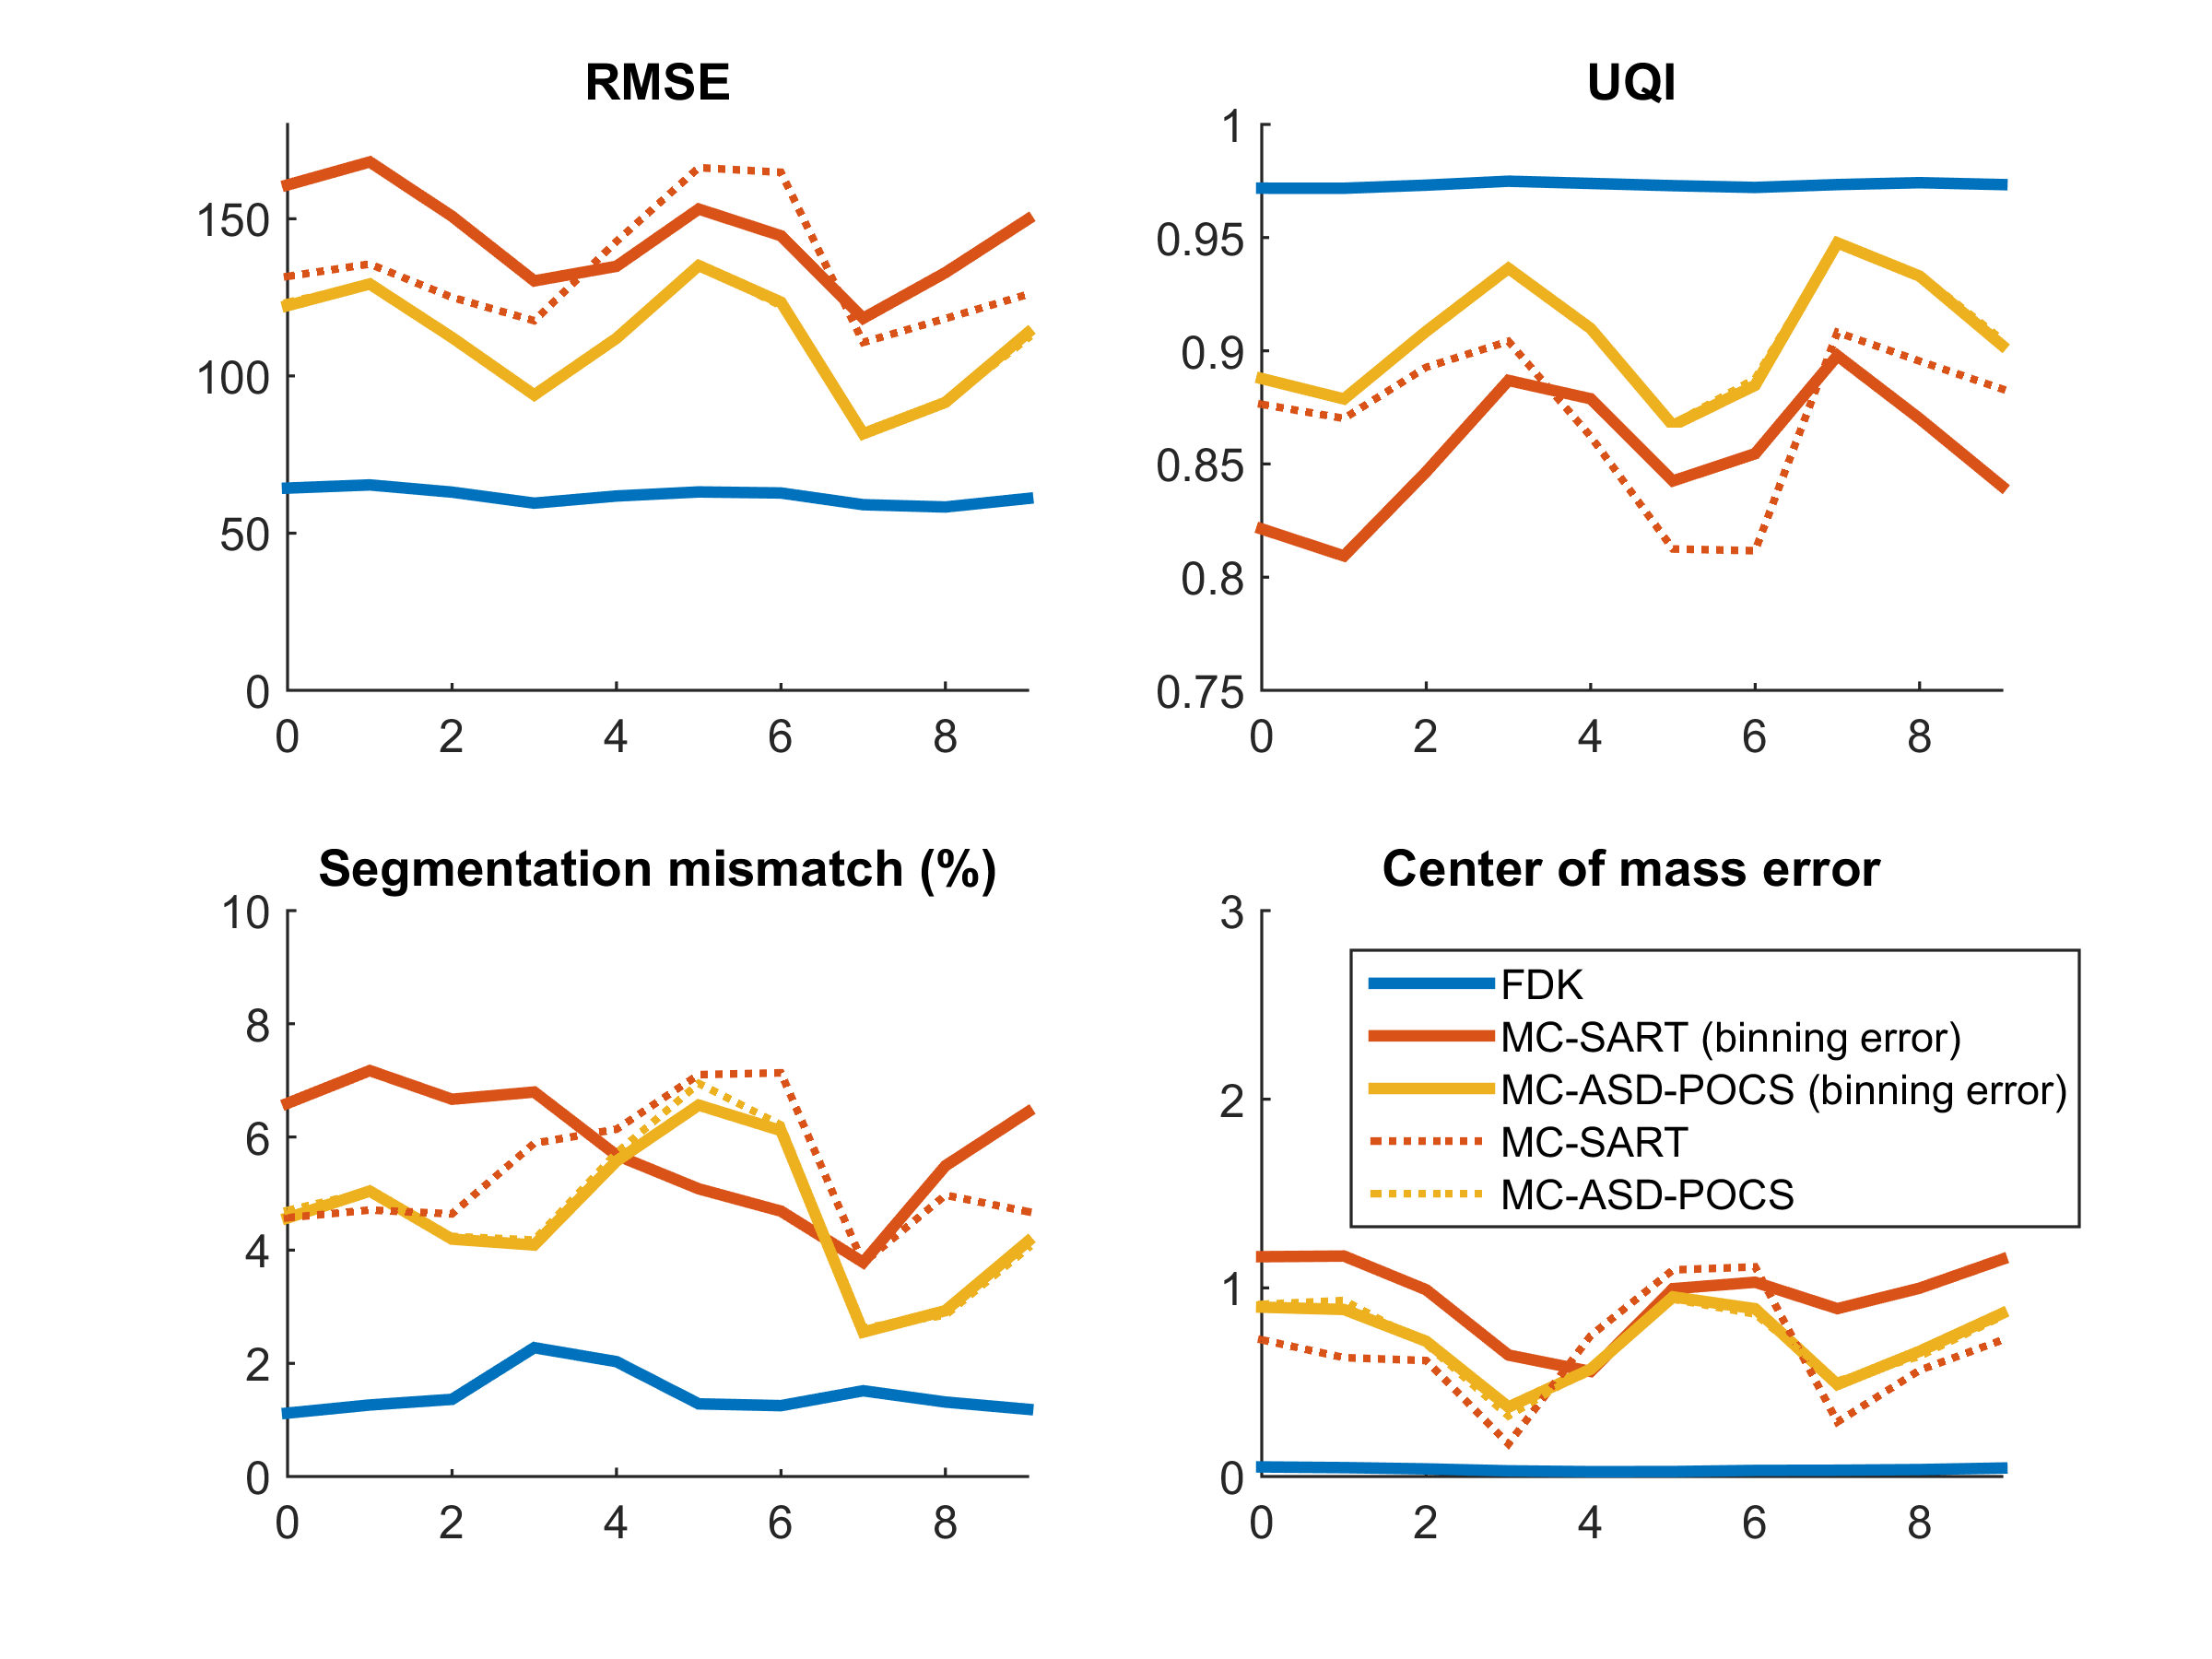
\includegraphics[width=0.9\textwidth]{accuracyMC/binningMCCBCTparams.png} 


\end{center}

\caption[Reconstruction quality comparison of motion compensation]{\label{fig:binMCCBCTquality}  Reconstruction quality comparison of 4D CBCT FDK, motion compensated methods (MC-SART and MC-ASD-POCS) and motion compensated methods with errors in projection binning (MC-SART (binning error) and MC-ASD-POCS (binning error)). Horizontal axis shows frame number and vertical axis the value of the quality parameter.} 
\end{figure}



\subsubsection{Only tumour motion information}

Nowadays clinically used breathing surrogates only give 1D signals of the breathing phase, and there are potential options for obtaining live 1D motion information of the tumour, such as implanted fiducials, ultrasound imaging\cite{western2015ultrasound} or electrical impedance tomography\cite{song2009non}\cite{pengpan2010motion} systems. Thus, evaluating the performance of the motion correction method for when only the motion of the tumour is known is crucial, as this would be the most likely introduction of the method to clinical cases, as the technology already exists. For the tests of this section, the DVFs are cropped to the same area as the tumour is for the quality evaluation plus 2 pixels in each direction, and set to zeros in the rest.

Figure \ref{fig:tumourMCCBCT3static} shows the difference between the motion compensation methods and the cropped DVF motion compensation for SART and ASD-POCS. Note that while the error is big in all of the image, the tumour are itself has no error. Similarly, figure \ref{fig:tumourMCCBCTquality} shows how the quality parameters are barely deteriorated after cropping most of the DVFs. This is an important result, as the motion is not only appearing in the tumour area for the specific X-rays that cross it, nevertheless the algorithm can discriminate the error and reconstruct accurately the tumour area, pushing the resultant motion errors outside the region of interest (observe box-like pattern around the tumour area).



\begin{figure}
\begin{center}

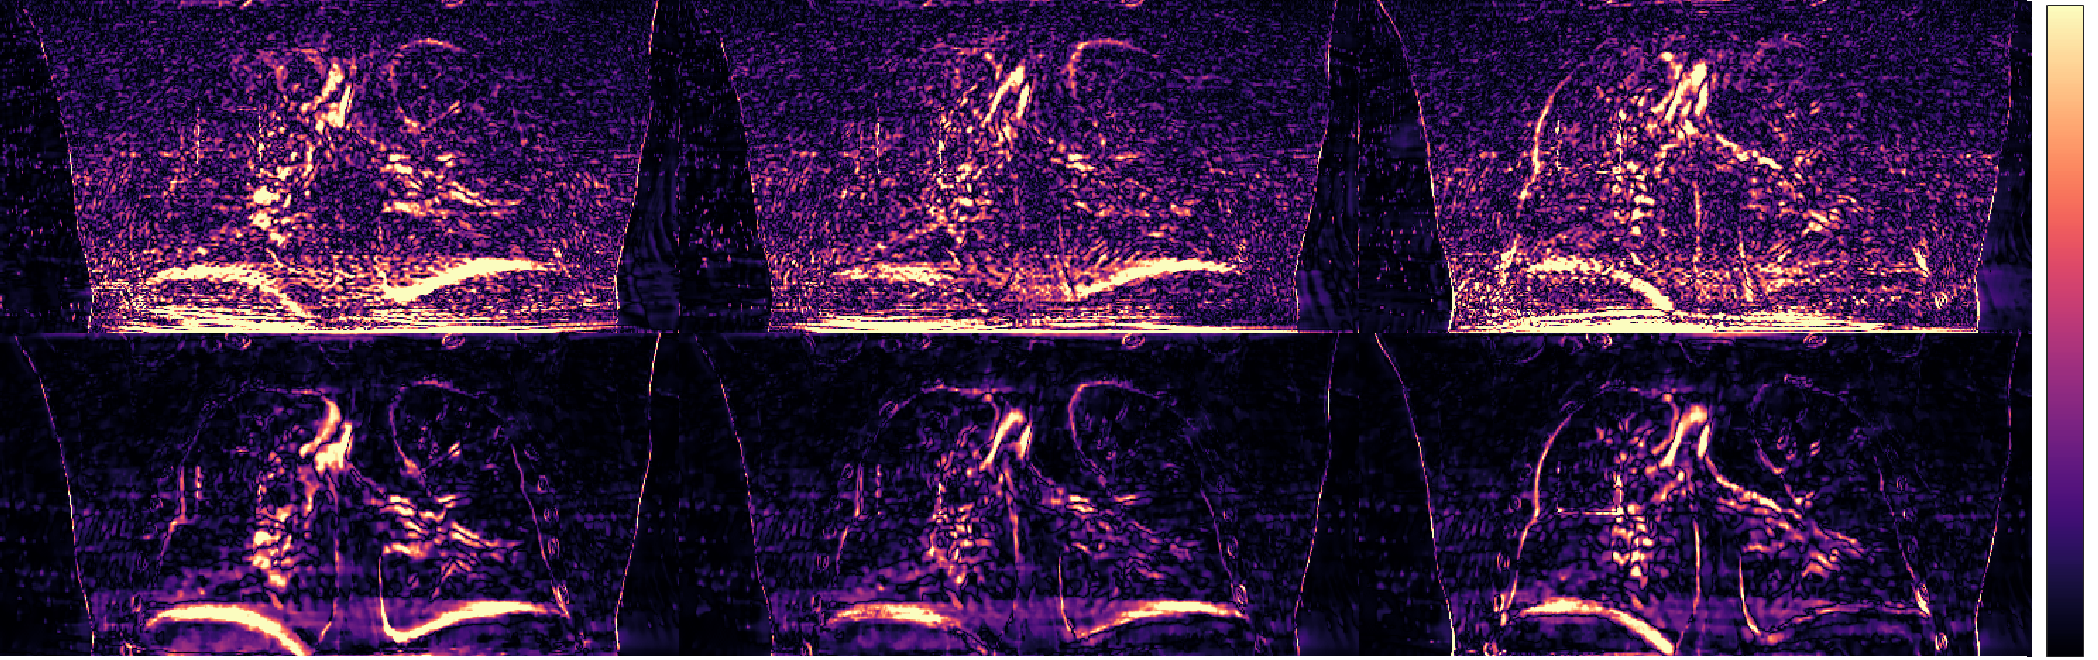
\includegraphics[width=\textwidth]{accuracyMC/difftumourMCCBCT3stage.png} 


\end{center}

\caption[Three difference frames of the  motion compensation methods with DVFs only in the tumour]{\label{fig:tumourMCCBCT3static} Absolute difference plots in frames (0,3 and 6) for the motion compensation methods with full DVFs or only DVFs if the tumour area, for SART and ASD-POCS, from top to bottom.  The colour scale is linear attenuation coefficient in the range [0-400].} 

\end{figure}


\begin{figure}
\begin{center}

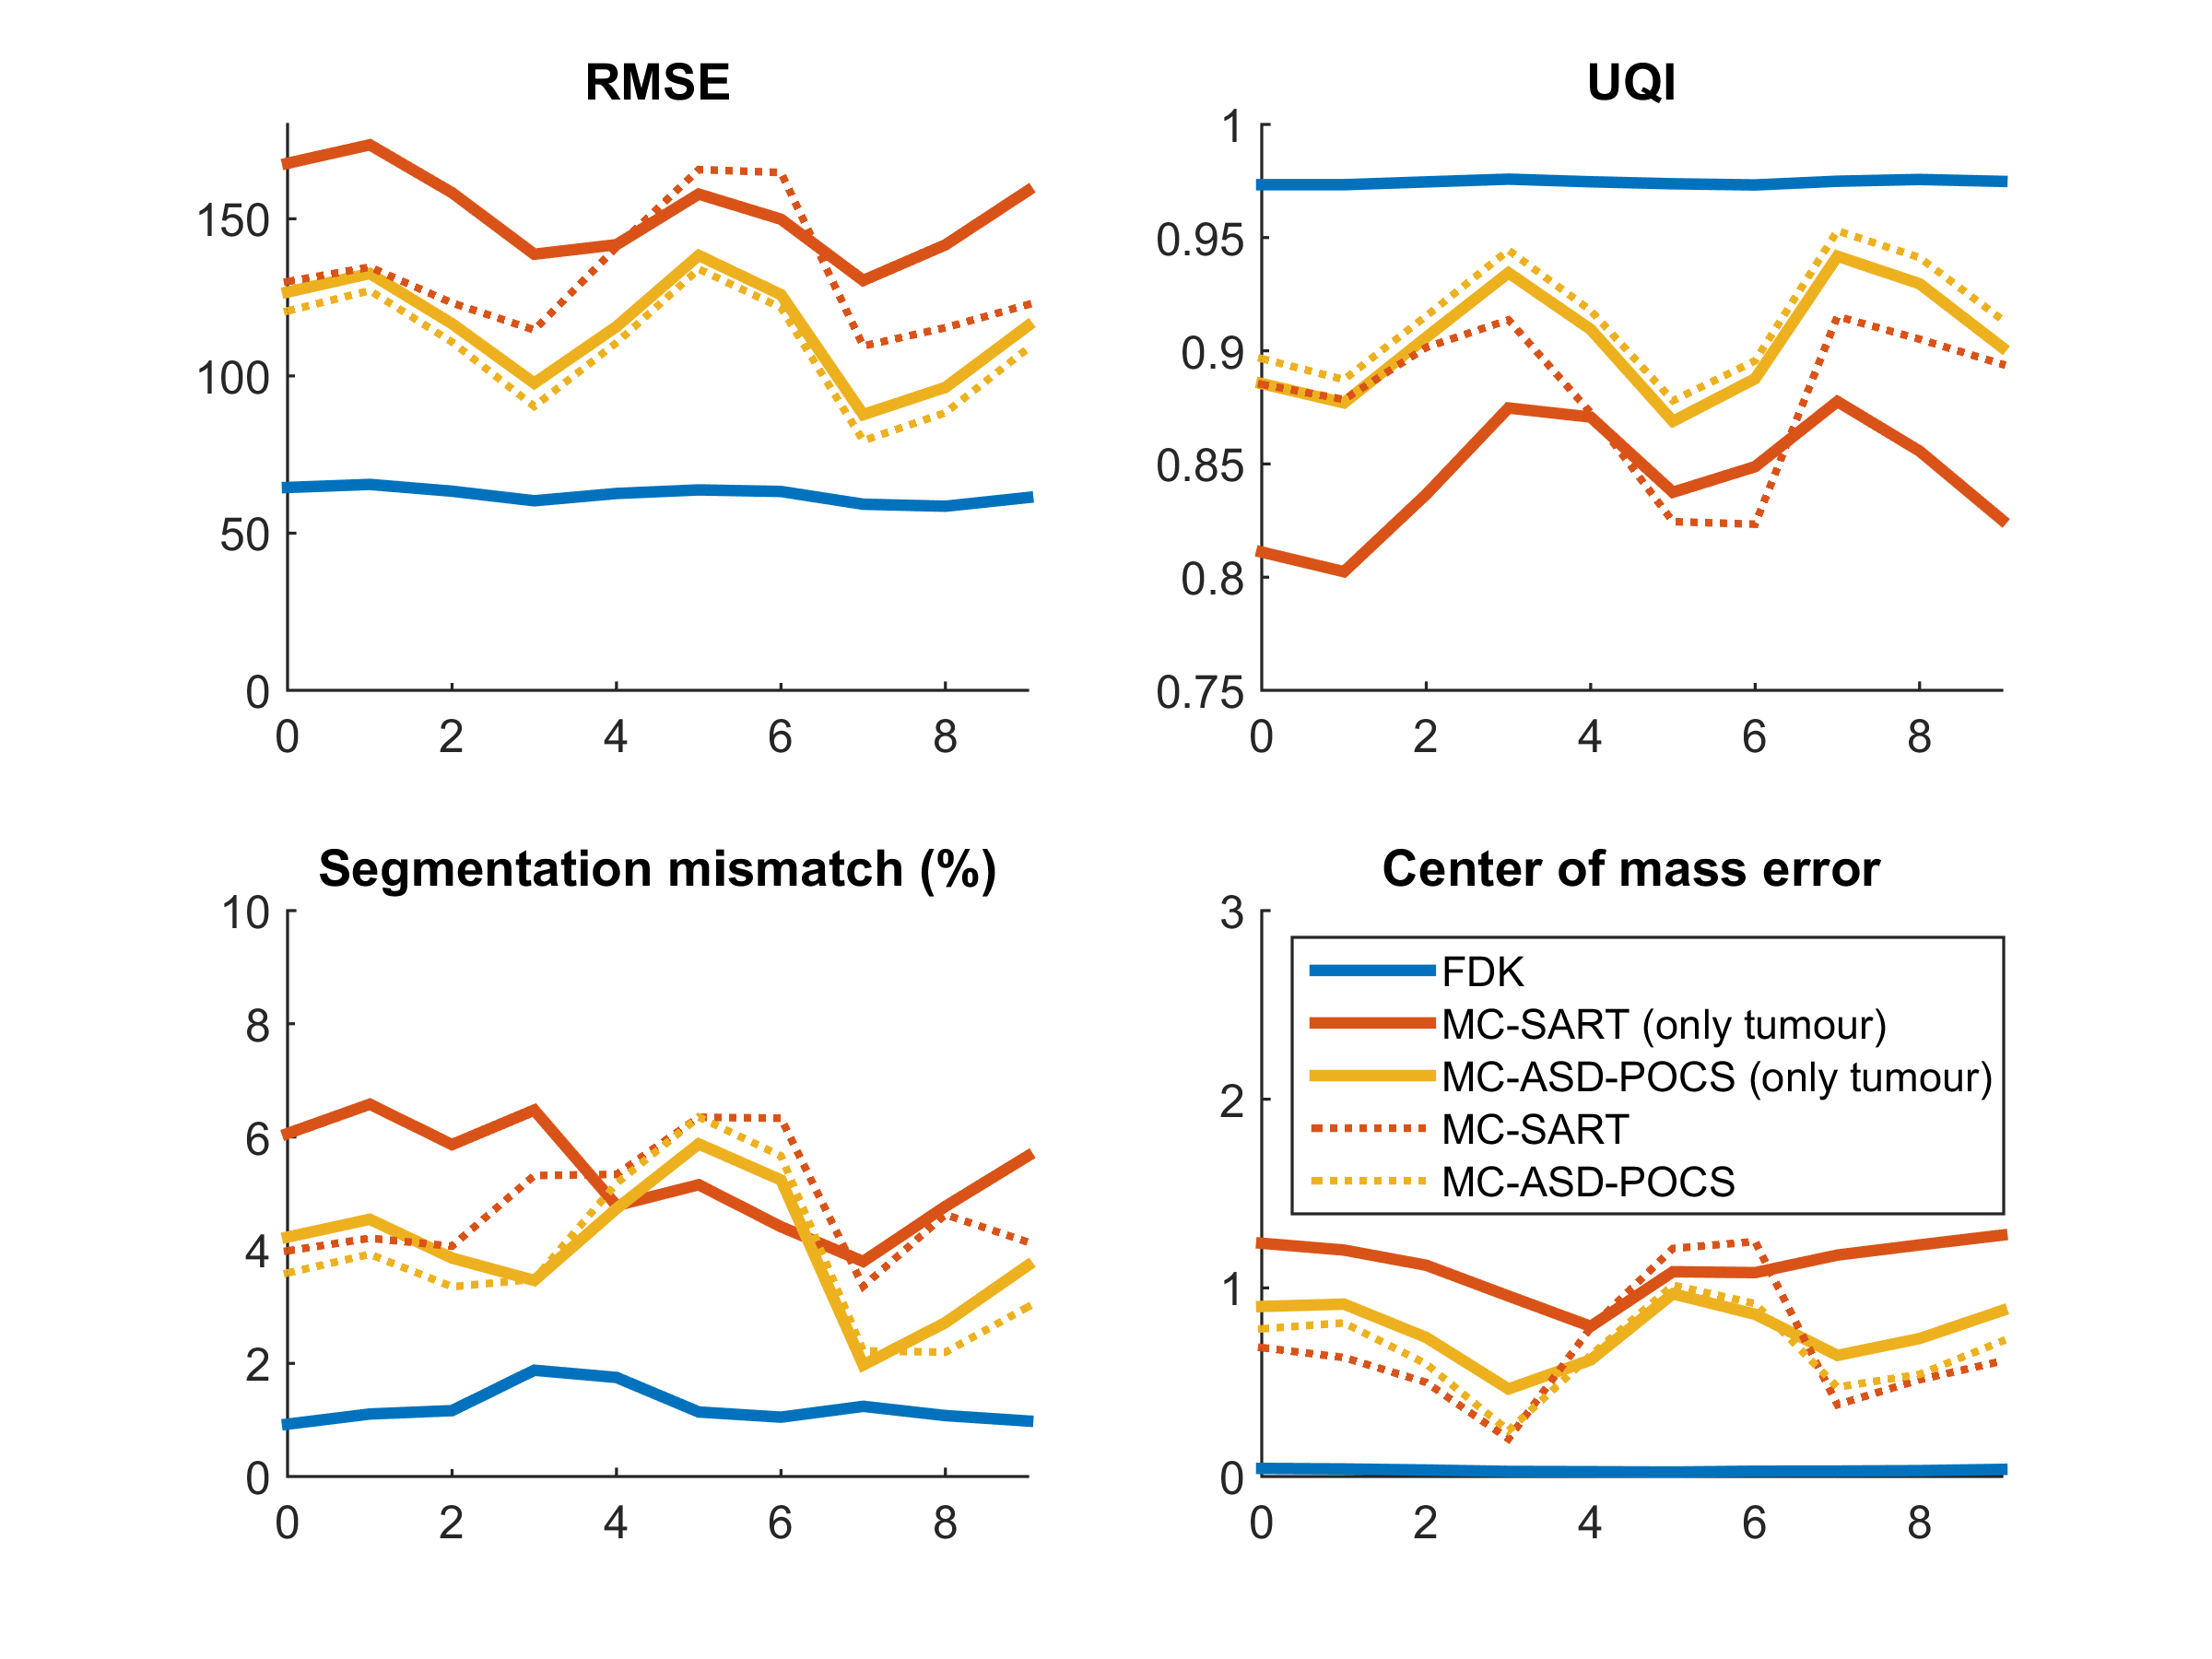
\includegraphics[width=0.9\textwidth]{accuracyMC/tumourMCCBCTparams.png} 


\end{center}

\caption[Reconstruction quality comparison of motion compensation]{\label{fig:tumourMCCBCTquality}  Reconstruction quality comparison of 4D CBCT FDK, motion compensated methods (MC-SART and MC-ASD-POCS) and motion compensated methods with only DVFs in the tumour (MC-SART (only tumour) and MC-ASD-POCS (only tumour)). Horizontal axis shows frame number and vertical axis the value of the quality parameter.} 
\end{figure}

\FloatBarrier
\section{Discussion}

This chapter has show the numerical accuracy of the motion compensated method proposed in this thesis as well as its comparison with standard 4D CBCT methods and its behaviour when the DVFs are suboptimal. First, iterative algorithms perform considerably better than FDK in 4D CBCT reconstruction, as others have already shown. The importance of choosing good algorithms for improved image quality is remarked. The results also hint that the motion compensated method can deliver 4D images using a tenth of the data needed for a 4D CBCT, thus reducing the dose to the patient by a significant amount. It should be also highlighted the robustness of the method to errors in DVFs, most importantly for binning errors and localized motion information. Binning errors are almost unavoidable in clinical cases, and the results clearly show the little effect it has in motion compensated iterative algorithms, especially in noise removing ones, such as ASD-POCS. This not only makes the algorithm robust to mislabels, but also to single breathing inhale-exhale phases that have different amplitude than expected, an effect that happens if a patient takes a deeper or shallower breath than usual. 

On top of that, the solid results for localized motion information is one of the strongest points in favour of the clinical application of this method, as it not only means that as long as the tumour position is known one can reconstruct it accurately, it also means that computationally fast methods for reconstruction can be easily designed. One of the biggest computational drawback is the need of memory storage of 3 times the size of the image for each different DVF, and equally 3 more texture memory samples in the projection operator, the biggest time constrain in the kernels. Only needing to perform this operations in a fraction of the image would speed the total time of the algorithm to  standard reconstruction in practical terms. Additionally, as previously mentioned, it is considerably more feasible to obtain real time location of the tumour only rather than the entire DVFs. 

The quality parameters are may need to be redefined to better evaluate the quality of the methods, however. RMSE and UQI are quite straightforward, but they are very limiting when evaluating the performance of reconstruction of something with spatial structure, as e.g. small random noise can increase their values significantly while maintaining the tumour delineation methods equally as accurate. When observing the tumour segmentation mismatch, the data shows that most of the mismatch is a missing 1 pixel wide surface around the motion compensated reconstruction, similar as in figure \ref{fig:tumourCC_err}. This hints that edge preserving algorithms may delineate the tumour better thus reducing most of the mismatch appearing in the motion compensated reconstruction. Alternatively smarter segmentation methods may also achieve a better delineation of the tumour thus showing a smaller error. The inter-method variation of the quality parameters is something also not expected on average. For example, most algorithms perform a bit worse around the frame 6, and this is highly likely due to DVS errors for this dataset on those frames. If the study were to be performed with multiple datasets, then the error is expected to be the same in all frames on average (assuming DVFs have the same average errors). 

This last observation highlights the biggest limit of the study shown in this chapter: it contains a single dataset. But this doesn't mean that the results are not valid, or that multiple datasets would show a different behaviour, as the cause of the change in quality of the reconstruction is clearly the caused by the algorithms used or the disturbances to DVFs introduced. The variation within each of the frames however, is not of big significance. However, if further use of the motion compensation methods for clinical use is desired, the results must be evaluated for multiple datasets. Additionally, the method should be evaluated with real CBCT projections, not only with simulated data.

This chapter strengthens the idea that motion compensated algorithms can have a significant improvement of image quality while reducing the dose to the patients by an order of magnitude, and that the existing tumour motion detection technologies may be enough information for the accurate usage of the algorithm on clinical cases. 




